%%%%%%%%%%%%%%%%%%%%%%%%%%%%%%%%%%%%%%%%%
% Beamer Presentation
% LaTeX Template
% Version 1.0 (10/11/12)
%
% This template has been downloaded from:
% http://www.LaTeXTemplates.com
%
% License:
% CC BY-NC-SA 3.0 (http://creativecommons.org/licenses/by-nc-sa/3.0/)
%
%%%%%%%%%%%%%%%%%%%%%%%%%%%%%%%%%%%%%%%%%

%----------------------------------------------------------------------------------------
%	PACKAGES AND THEMES
%----------------------------------------------------------------------------------------

\documentclass{beamer}

\mode<presentation> {

% The Beamer class comes with a number of default slide themes
% which change the colors and layouts of slides. Below this is a list
% of all the themes, uncomment each in turn to see what they look like.

%\usetheme{default}
%\usetheme{AnnArbor}
%\usetheme{Antibes}
%\usetheme{Bergen}
%\usetheme{Berkeley}
%\usetheme{Berlin}
%\usetheme{Boadilla}
%\usetheme{CambridgeUS}
%\usetheme{Copenhagen}
%\usetheme{Darmstadt}
%\usetheme{Dresden}
%\usetheme{Frankfurt}
%\usetheme{Goettingen}
%\usetheme{Hannover}
%\usetheme{Ilmenau}
%\usetheme{JuanLesPins}
%\usetheme{Luebeck}
%\usetheme{Madrid}
%\usetheme{Malmoe}
%\usetheme{Marburg}
%\usetheme{Montpellier}
\usetheme{PaloAlto}
%\usetheme{Pittsburgh}
%\usetheme{Rochester}
%\usetheme{Singapore}
%\usetheme{Szeged}
%\usetheme{Warsaw}

% As well as themes, the Beamer class has a number of color themes
% for any slide theme. Uncomment each of these in turn to see how it
% changes the colors of your current slide theme.

%\usecolortheme{albatross}
%\usecolortheme{beaver}
%\usecolortheme{beetle}
%\usecolortheme{crane}
\usecolortheme{dolphin}
%\usecolortheme{dove}
%\usecolortheme{fly}
%\usecolortheme{lily}
%\usecolortheme{orchid}
%\usecolortheme{rose}
%\usecolortheme{seagull}
%\usecolortheme{seahorse}
%\usecolortheme{whale}
%\usecolortheme{wolverine}

\usefonttheme{structurebold}

\setbeamertemplate{footline} % To remove the footer line in all slides uncomment this line
%\setbeamertemplate{footline}[page number] % To replace the footer line in all slides with a simple slide count uncomment this line

\setbeamertemplate{navigation symbols}{} % To remove the navigation symbols from the bottom of all slides uncomment this line
}

\setbeamertemplate{items}[square]

\usepackage{graphicx} % Allows including images
\usepackage{booktabs} % Allows the use of \toprule, \midrule and \bottomrule in tables
\usepackage{textpos} % Package for text positioning
\usepackage{media9}


%----------------------------------------------------------------------------------------
%	TITLE PAGE
%----------------------------------------------------------------------------------------

\title[Microrod Lasing]{Toward Chip Integrated Ultra-Low-Noise Lasing Using a Microrod Resonator} % The short title appears at the bottom of every slide, the full title is only on the title page

\author[J. Becker]{Joe Becker \\
\scriptsize{W. Loh, F. Baynes, D. Cole, F. Quinlan, H. Lee,\\
K. Vahala, S. Papp, S. Diddams}} % Your name 

\titlegraphic{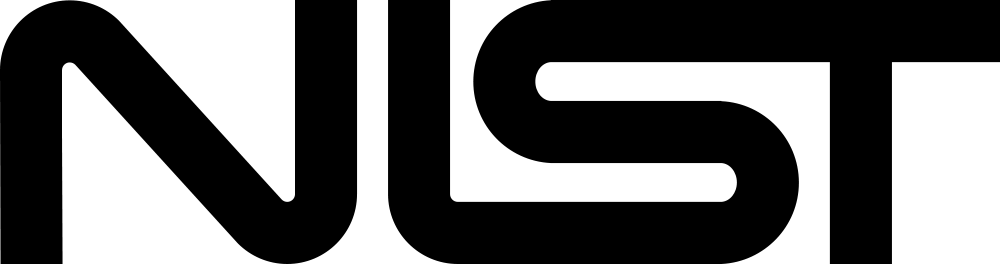
\includegraphics[height=0.8cm]{Images/NIST_logo.png}}

\institute[NIST] % Your institution as it will appear on the bottom of every slide, may be shorthand to save space
{
National Institute of Standards and Technology\\ % Your institution for the title page
\medskip
\textit{Joe.Becker@nist.gov} % Your email address
}

\date{April 15, 2015} % Date, can be changed to a custom date

\setbeamertemplate{section in toc}{\inserttocsection}

%\setbeamercolor{block title}{fg=black, bg=yellow}
%\setbeamercolor{title}{fg=black, bg=yellow}
%\setbeamercolor{frametitle}{fg=black, bg=yellow}
%\setbeamercolor{title in sidebar}{use=normal text,fg=black}
%\setbeamercolor{author in sidebar}{use=normal text,fg=black}
%\setbeamercolor{section in sidebar}{use=normal text,fg=black}
%\setbeamercolor{section in sidebar shaded}{use=normal text,fg=black!75!white}
%\setbeamercolor{item}{fg=black}

%titlepage logo
\addtobeamertemplate{frametitle}{}{
\begin{textblock*}{3cm}(-2cm,-1cm)
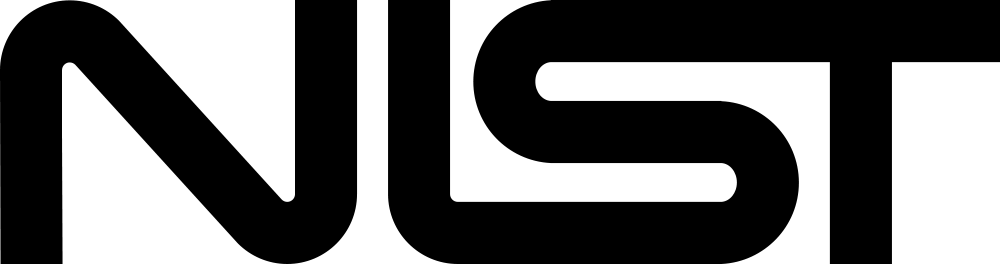
\includegraphics[width=1.4cm,keepaspectratio]{Images/NIST_logo.png}
\end{textblock*}}


\begin{document}

\begin{frame}
\titlepage % Print the title page as the first slide
\end{frame}

%%%%%%%%%PRESENTATION SLIDES%%%%%%%%

\section{Background} 
\begin{frame}\frametitle{Current Laser Technology}
As lasers increase in stability they increase in size.
\includegraphics<1>[width=0.95\textwidth]{Images/Current_Laser1.png}
\includegraphics<2>[width=0.95\textwidth]{Images/Current_Laser2.png}
\end{frame}

\begin{frame}{Whispering Gallery Mode Resonators}
\centering
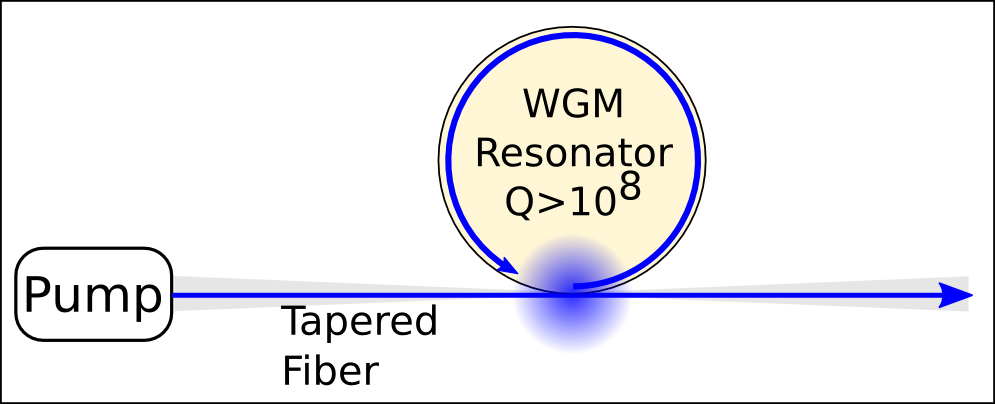
\includegraphics[width=0.7\textwidth]{Images/WGM_Resonator_Fig.png}
\begin{columns}

\column{0.3\textwidth}
\begin{block}{Silica Microdisk}
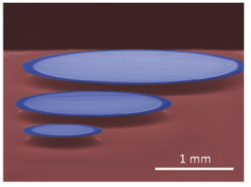
\includegraphics[width=0.5\textwidth]{Images/Wedge_Microdisk.png}
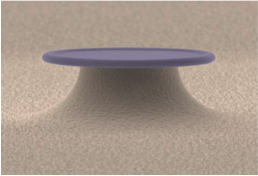
\includegraphics[width=0.5\textwidth]{Images/Microtoroid.png}

\scriptsize
H. Lee, Nature Photon, 2012
\end{block}

\column{0.3\textwidth}
\begin{block}{Silica Microrod}
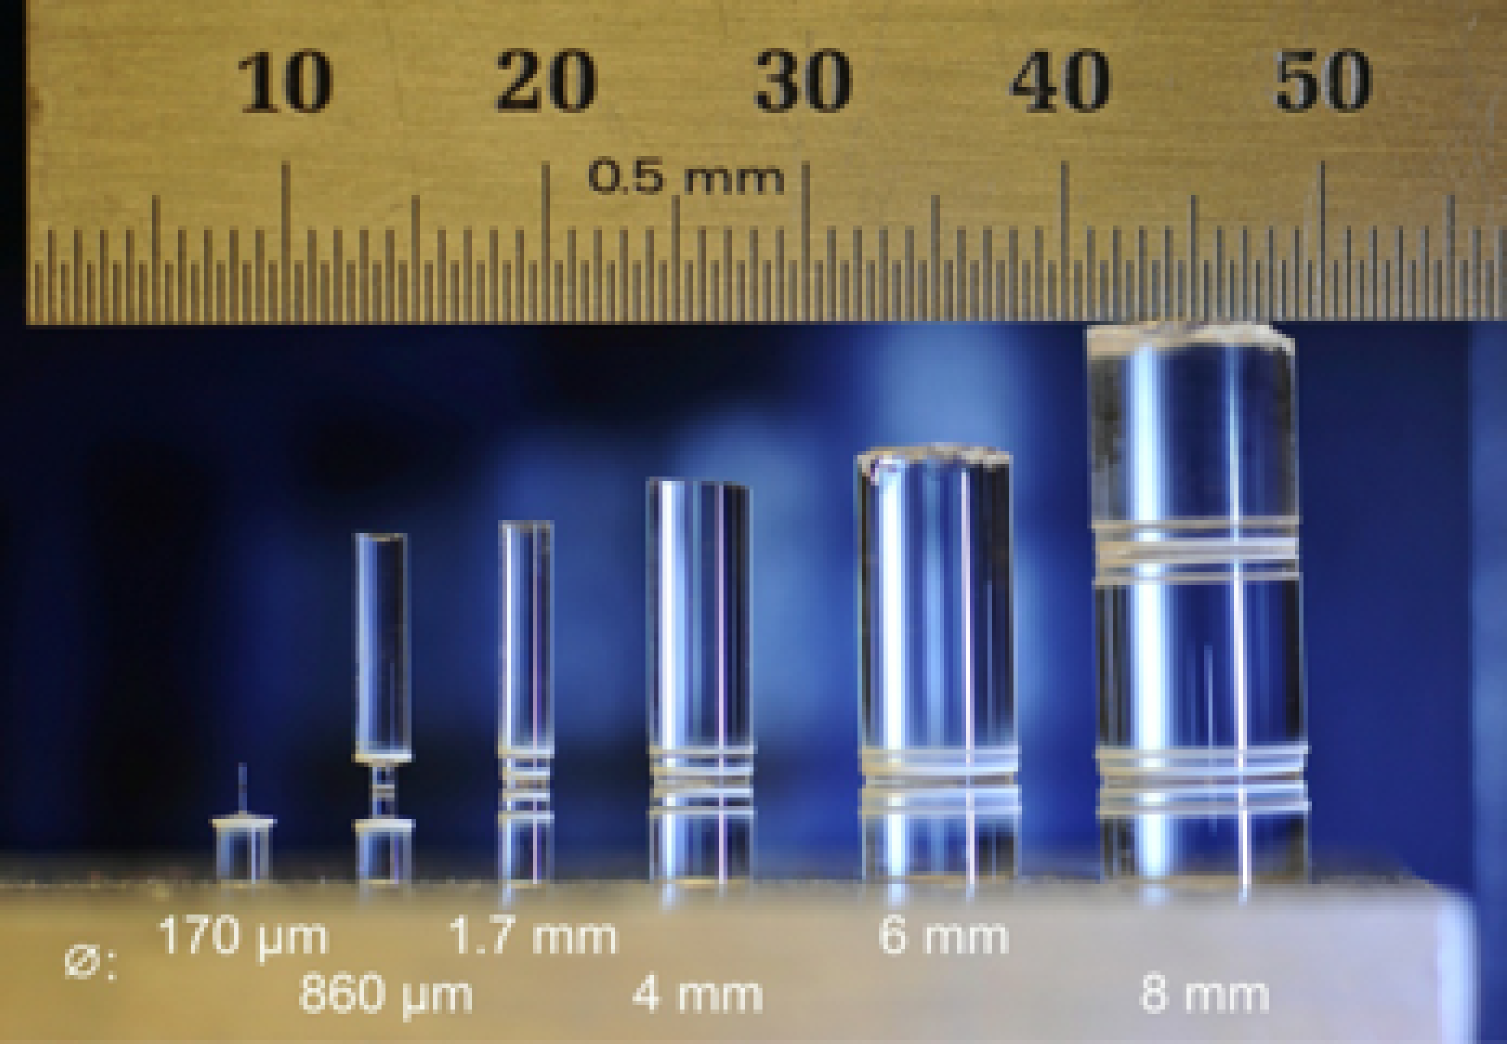
\includegraphics[width=1.0\textwidth]{Images/Microrods.png}

\scriptsize
P. Del'Haye, APL, 2013
\end{block}

\column{0.3\textwidth}
\begin{block}{CaF$_2$ Resonator}
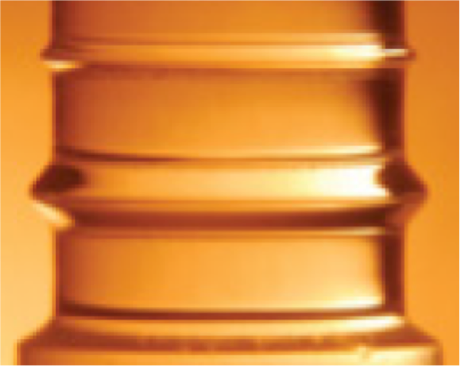
\includegraphics[width=1.0\textwidth]{Images/CaF2_resonator.png}

\scriptsize
J. Hofer, PRA, 2010\\
W. Liang, Opt Lett., 2011
\end{block}
\end{columns}
\end{frame}

\begin{frame}\frametitle{Brillouin Lasers}
\begin{columns}
\column{0.55\textwidth}
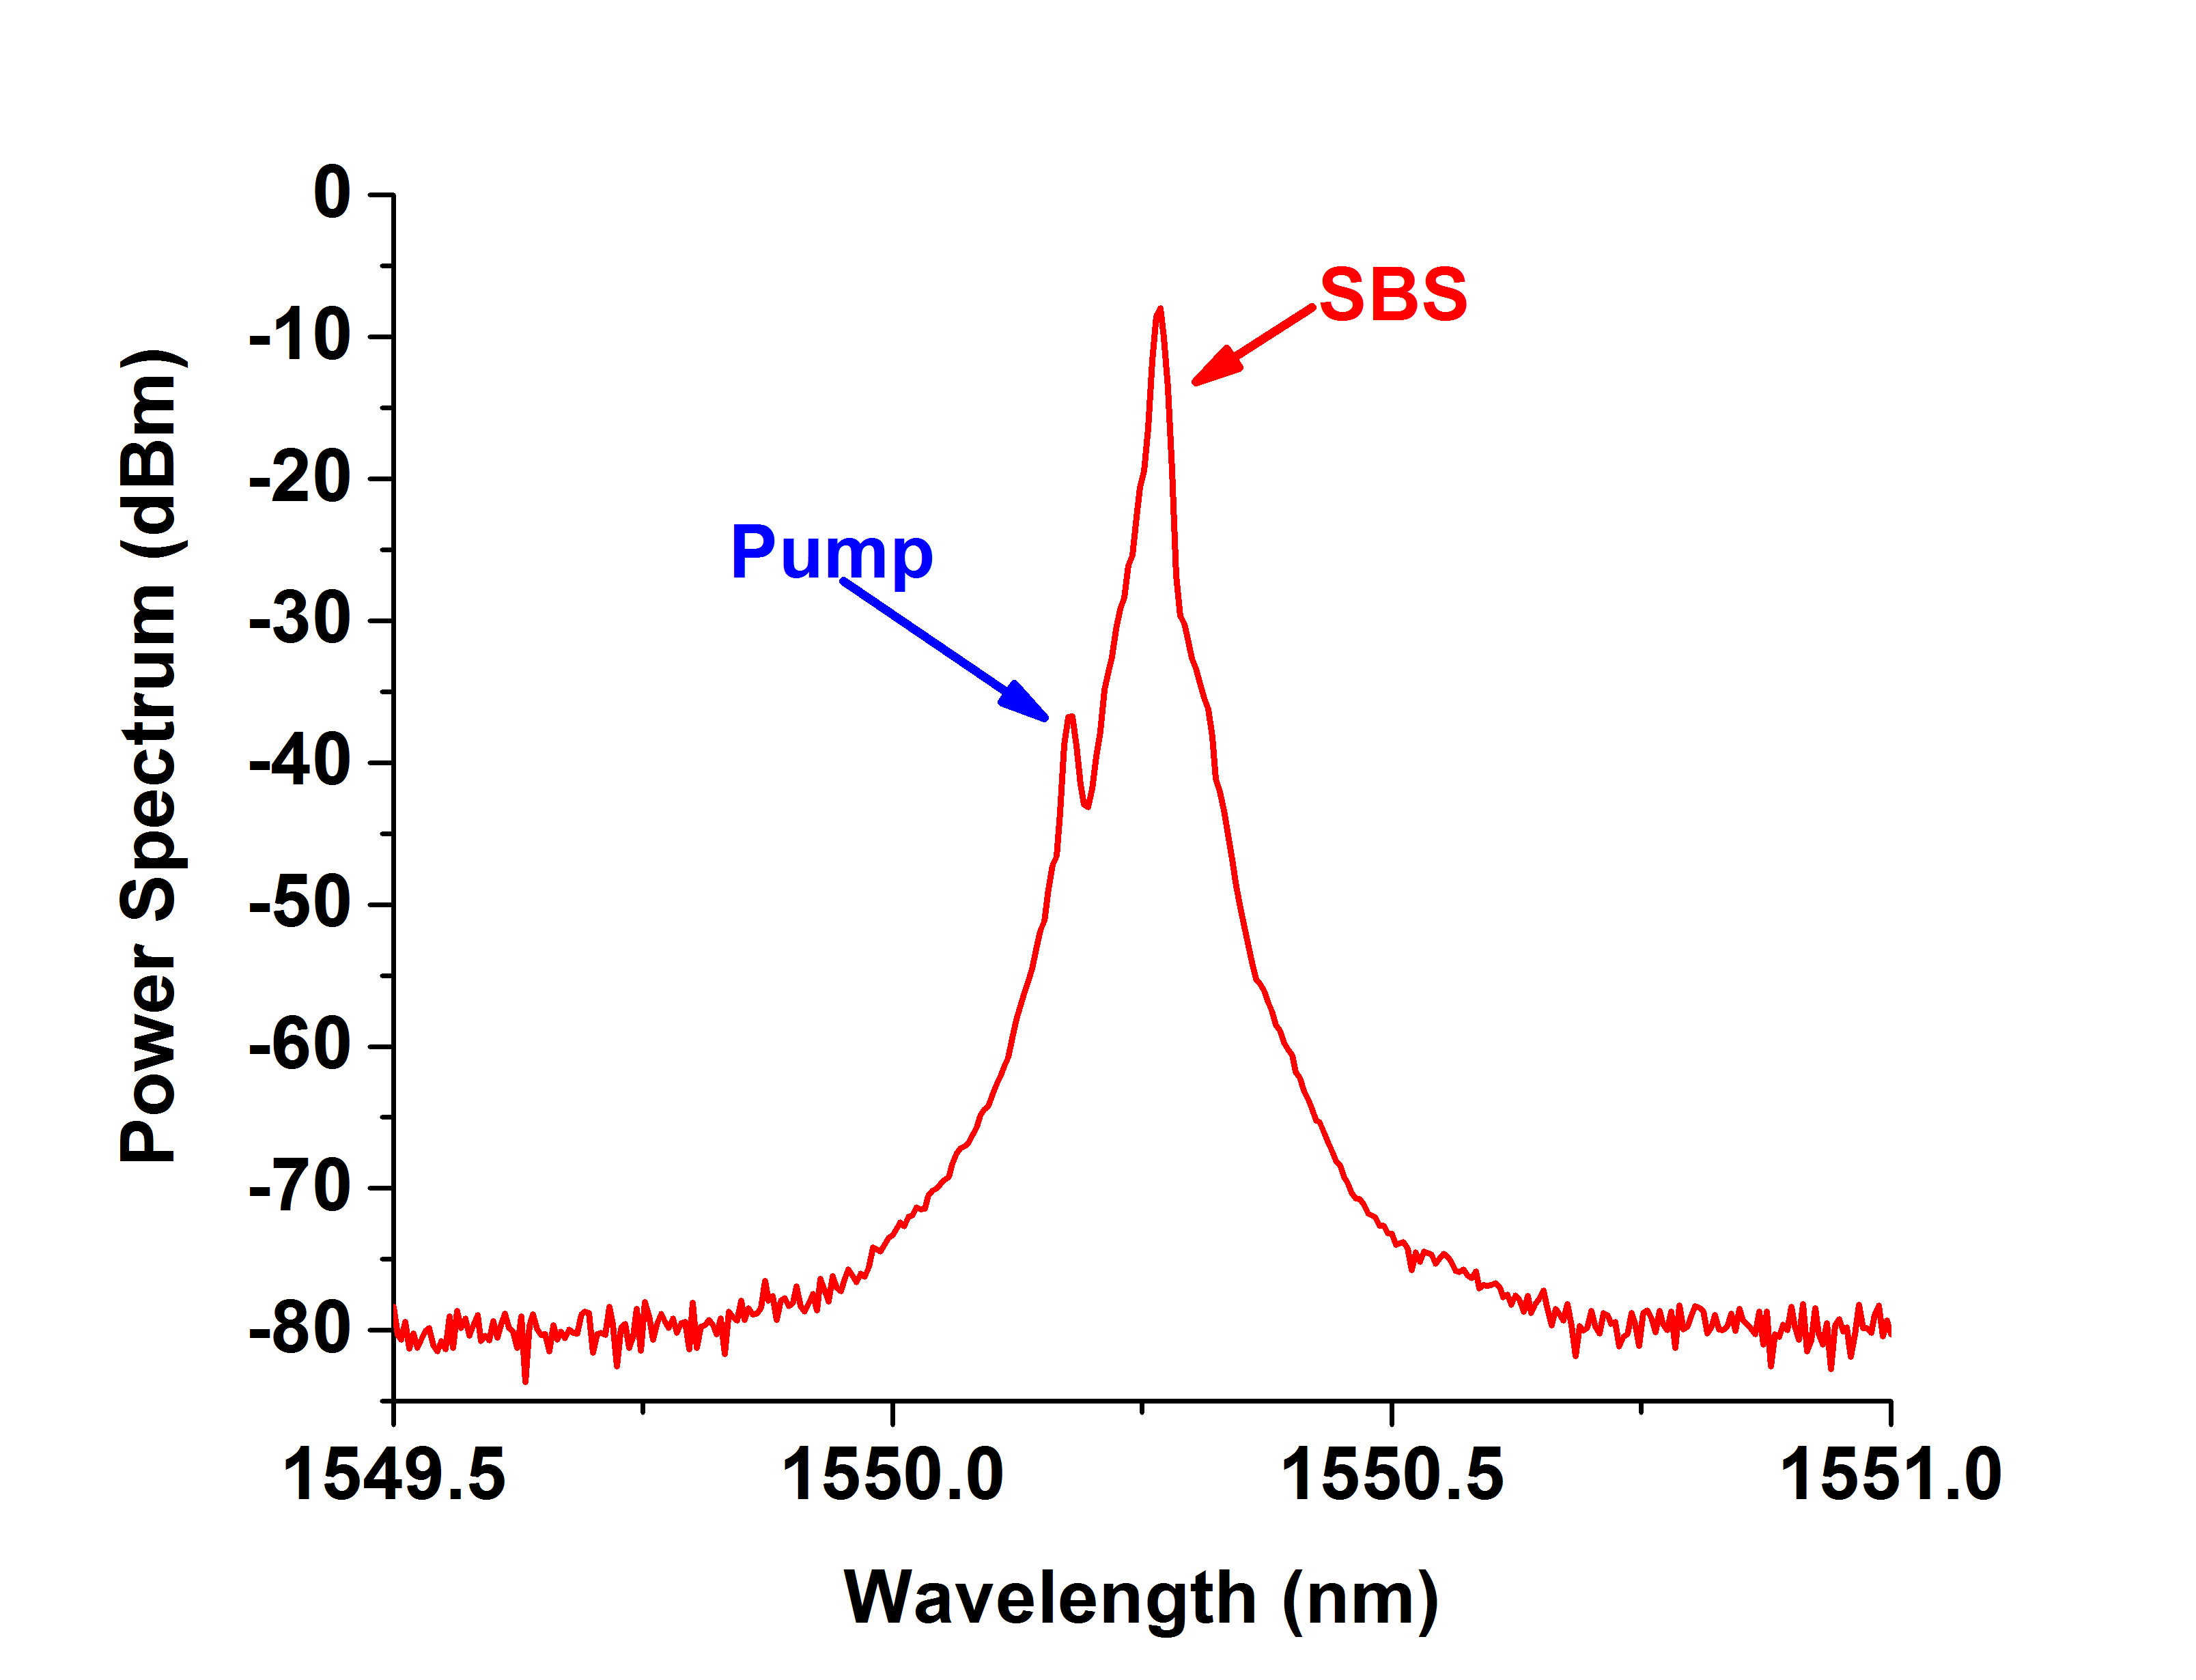
\includegraphics[width=1.0\textwidth,keepaspectratio]{Images/SBS_Optical_Spectrum.png}\\
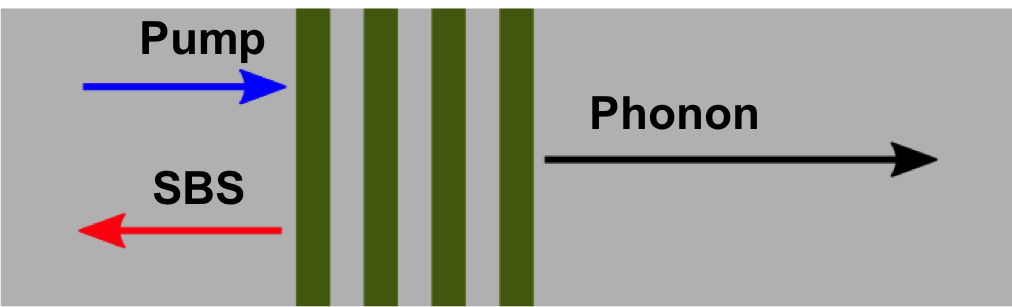
\includegraphics[width=1.0\textwidth,keepaspectratio]{Images/SBS_Figure.png}
\column{0.47\textwidth}
\begin{block}{Gain Process}
\begin{itemize}
\item Brillouin scattering is a nonlinear process where a photon scatters off of a propagating phonon resulting in a backscattered photon
which Doppler shifted due to the movement of the phonon.
\item SBS and pump fields interfere to drive the phonons to stimulate additional Brillouin scattering.
\end{itemize}
\end{block}
\end{columns}
\end{frame}

\begin{frame}\frametitle{Why SBS Lasers?}
\begin{columns}
\column{0.5\textwidth}
Because they have a high signal to noise ratio!
\column{0.5\textwidth}
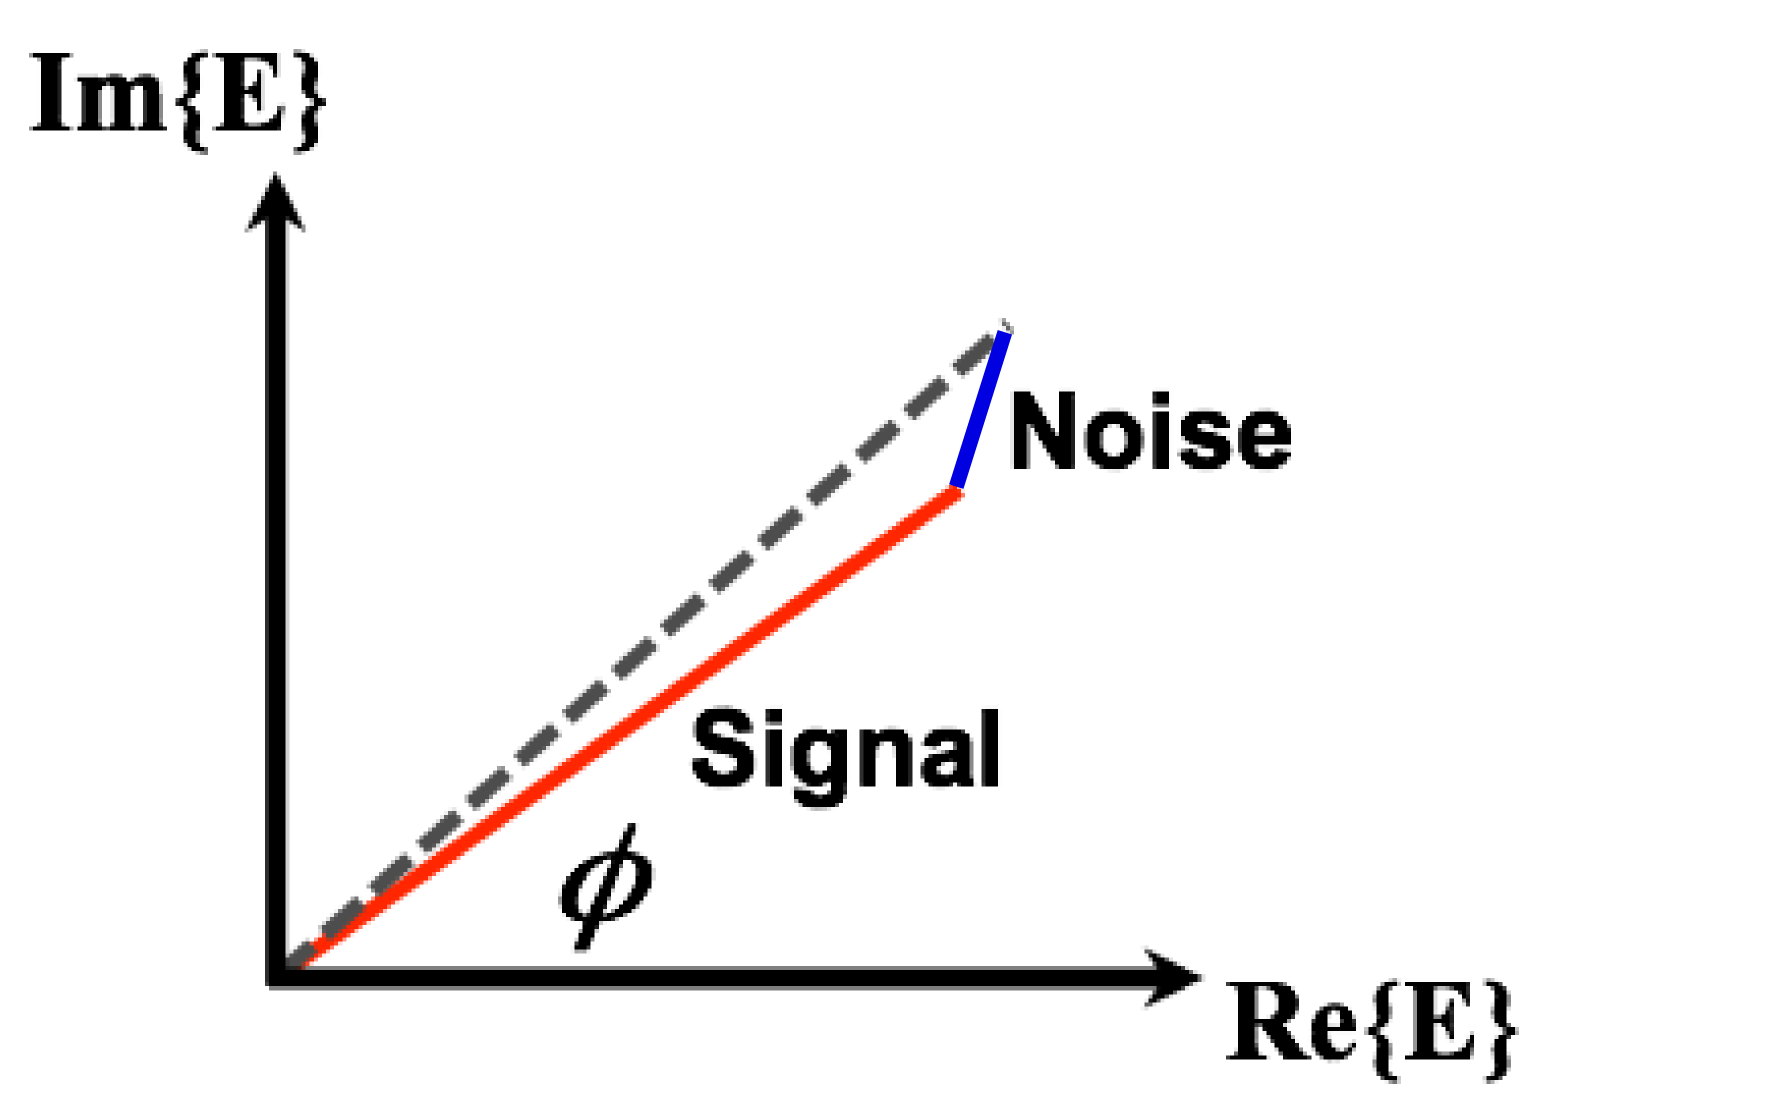
\includegraphics[width=1.0\textwidth]{Images/SBS_Noise.png}
\end{columns}

\begin{block}{SBS Laser Noise}
\begin{columns}
\column{0.45\textwidth}
SBS laser noise is governed by thermal fluctuations which are much larger than the energy of the phonons.  
$$\frac{h\nu}{k_B T}<<1$$
\column{0.45\textwidth}
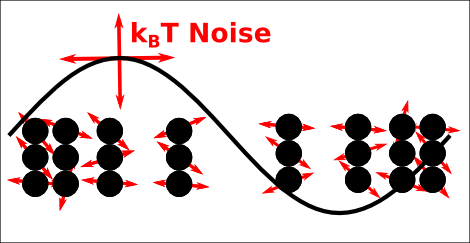
\includegraphics[width=1.0\textwidth]{Images/Thermal_Noise.png}
\end{columns}
\end{block}
\end{frame}

\begin{frame}\frametitle{SBS Lasers in Microresonators}
Microresonators are a prime candidate for creating ultra-low-noise lasers using SBS, because of their ultra-high Q.
\begin{columns}
\column{0.5\textwidth}
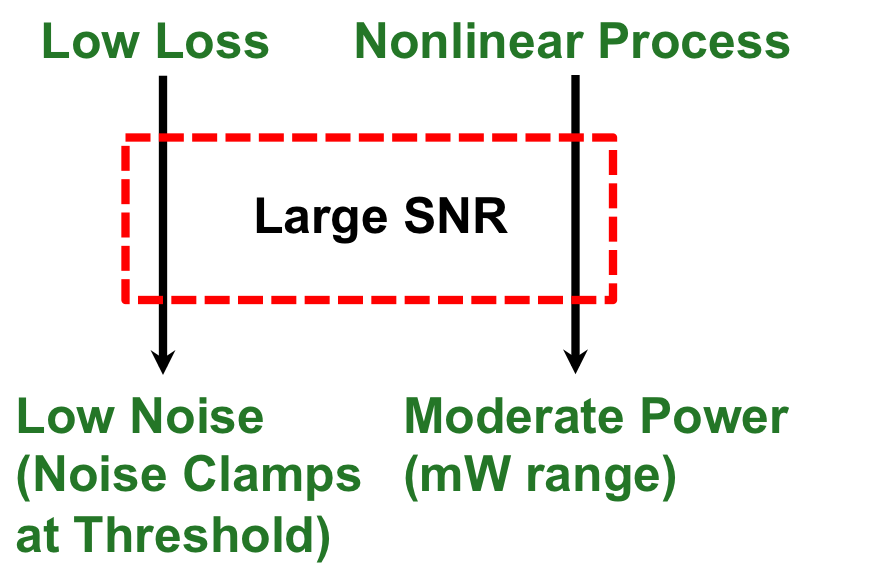
\includegraphics[width=1.0\textwidth]{Images/SBS_Microres_SNR.png}
\column{0.5\textwidth}
\begin{itemize}
\item Their low loss means a lower gain level at steady state operation.
\item Lower gain threshold allows for less thermal noise to be added to the signal.
\item Non-linear process lead to high signal power.

\end{itemize}
\end{columns}
\end{frame}

\begin{frame}\frametitle{SBS Laser in Microdisk}
\begin{columns}
\column{0.5\textwidth}
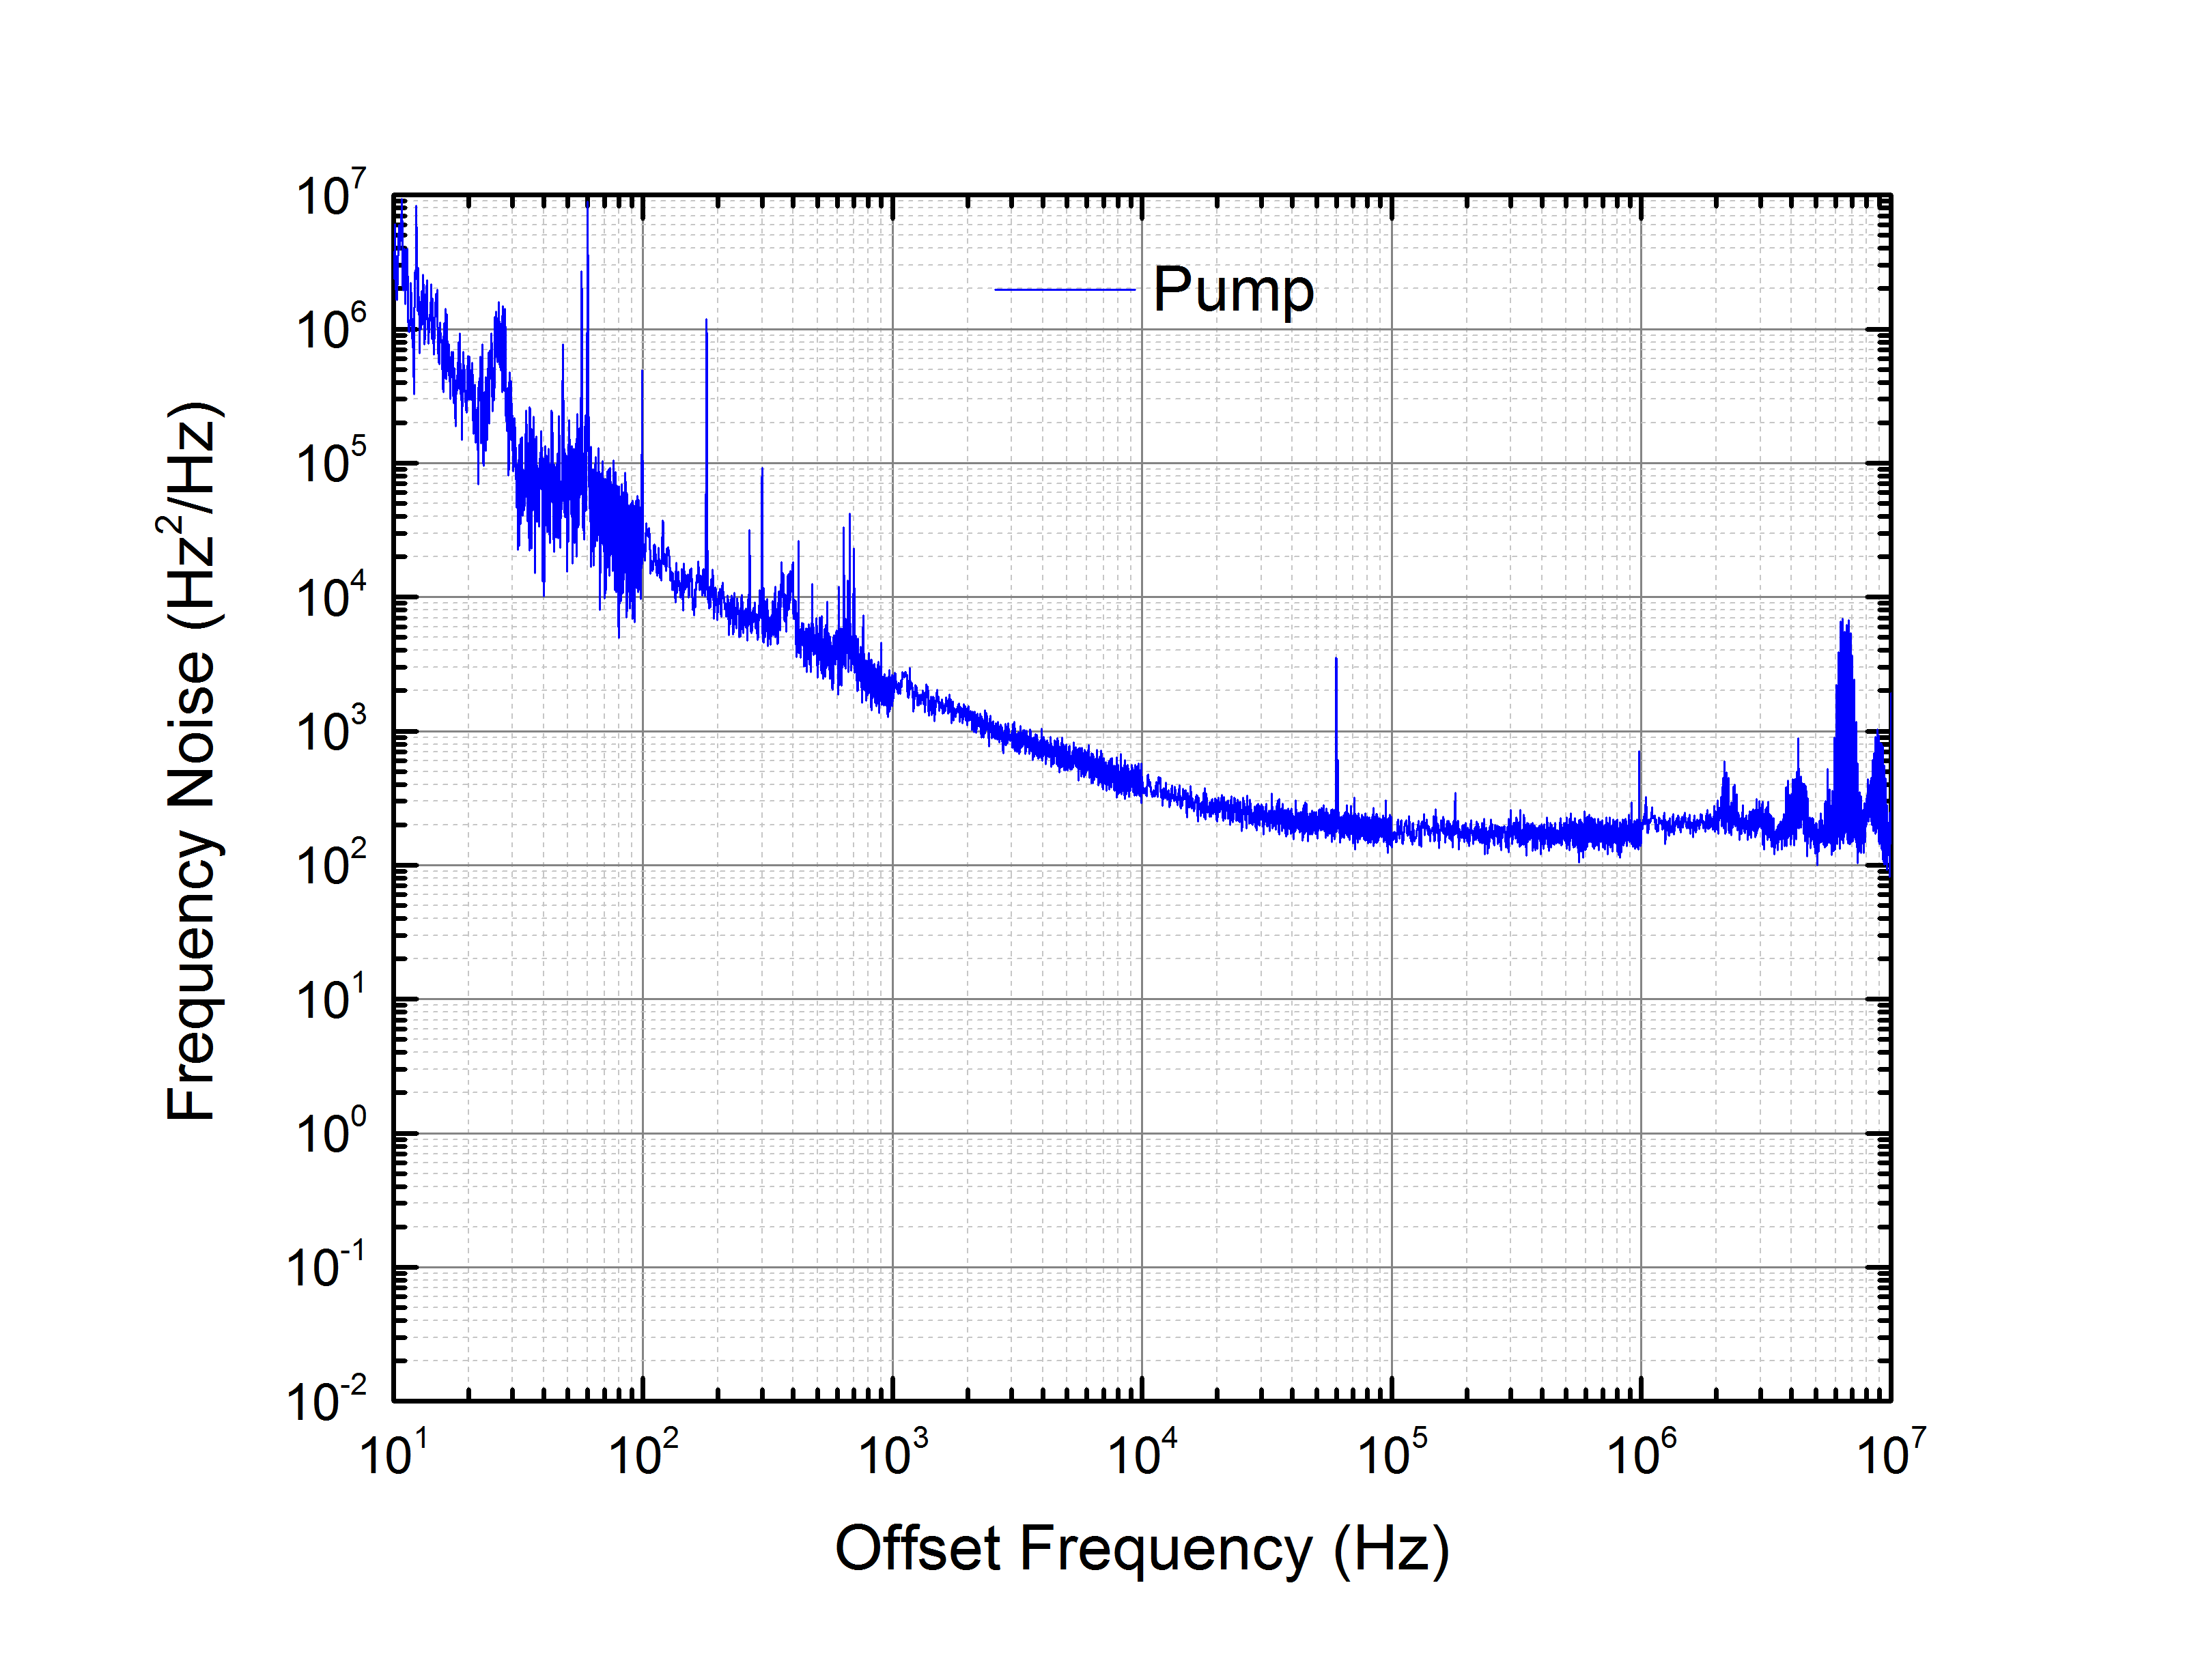
\includegraphics[width=1.0\textwidth]{Images/Freq_Noise_Comparison_Plot1.png}\\
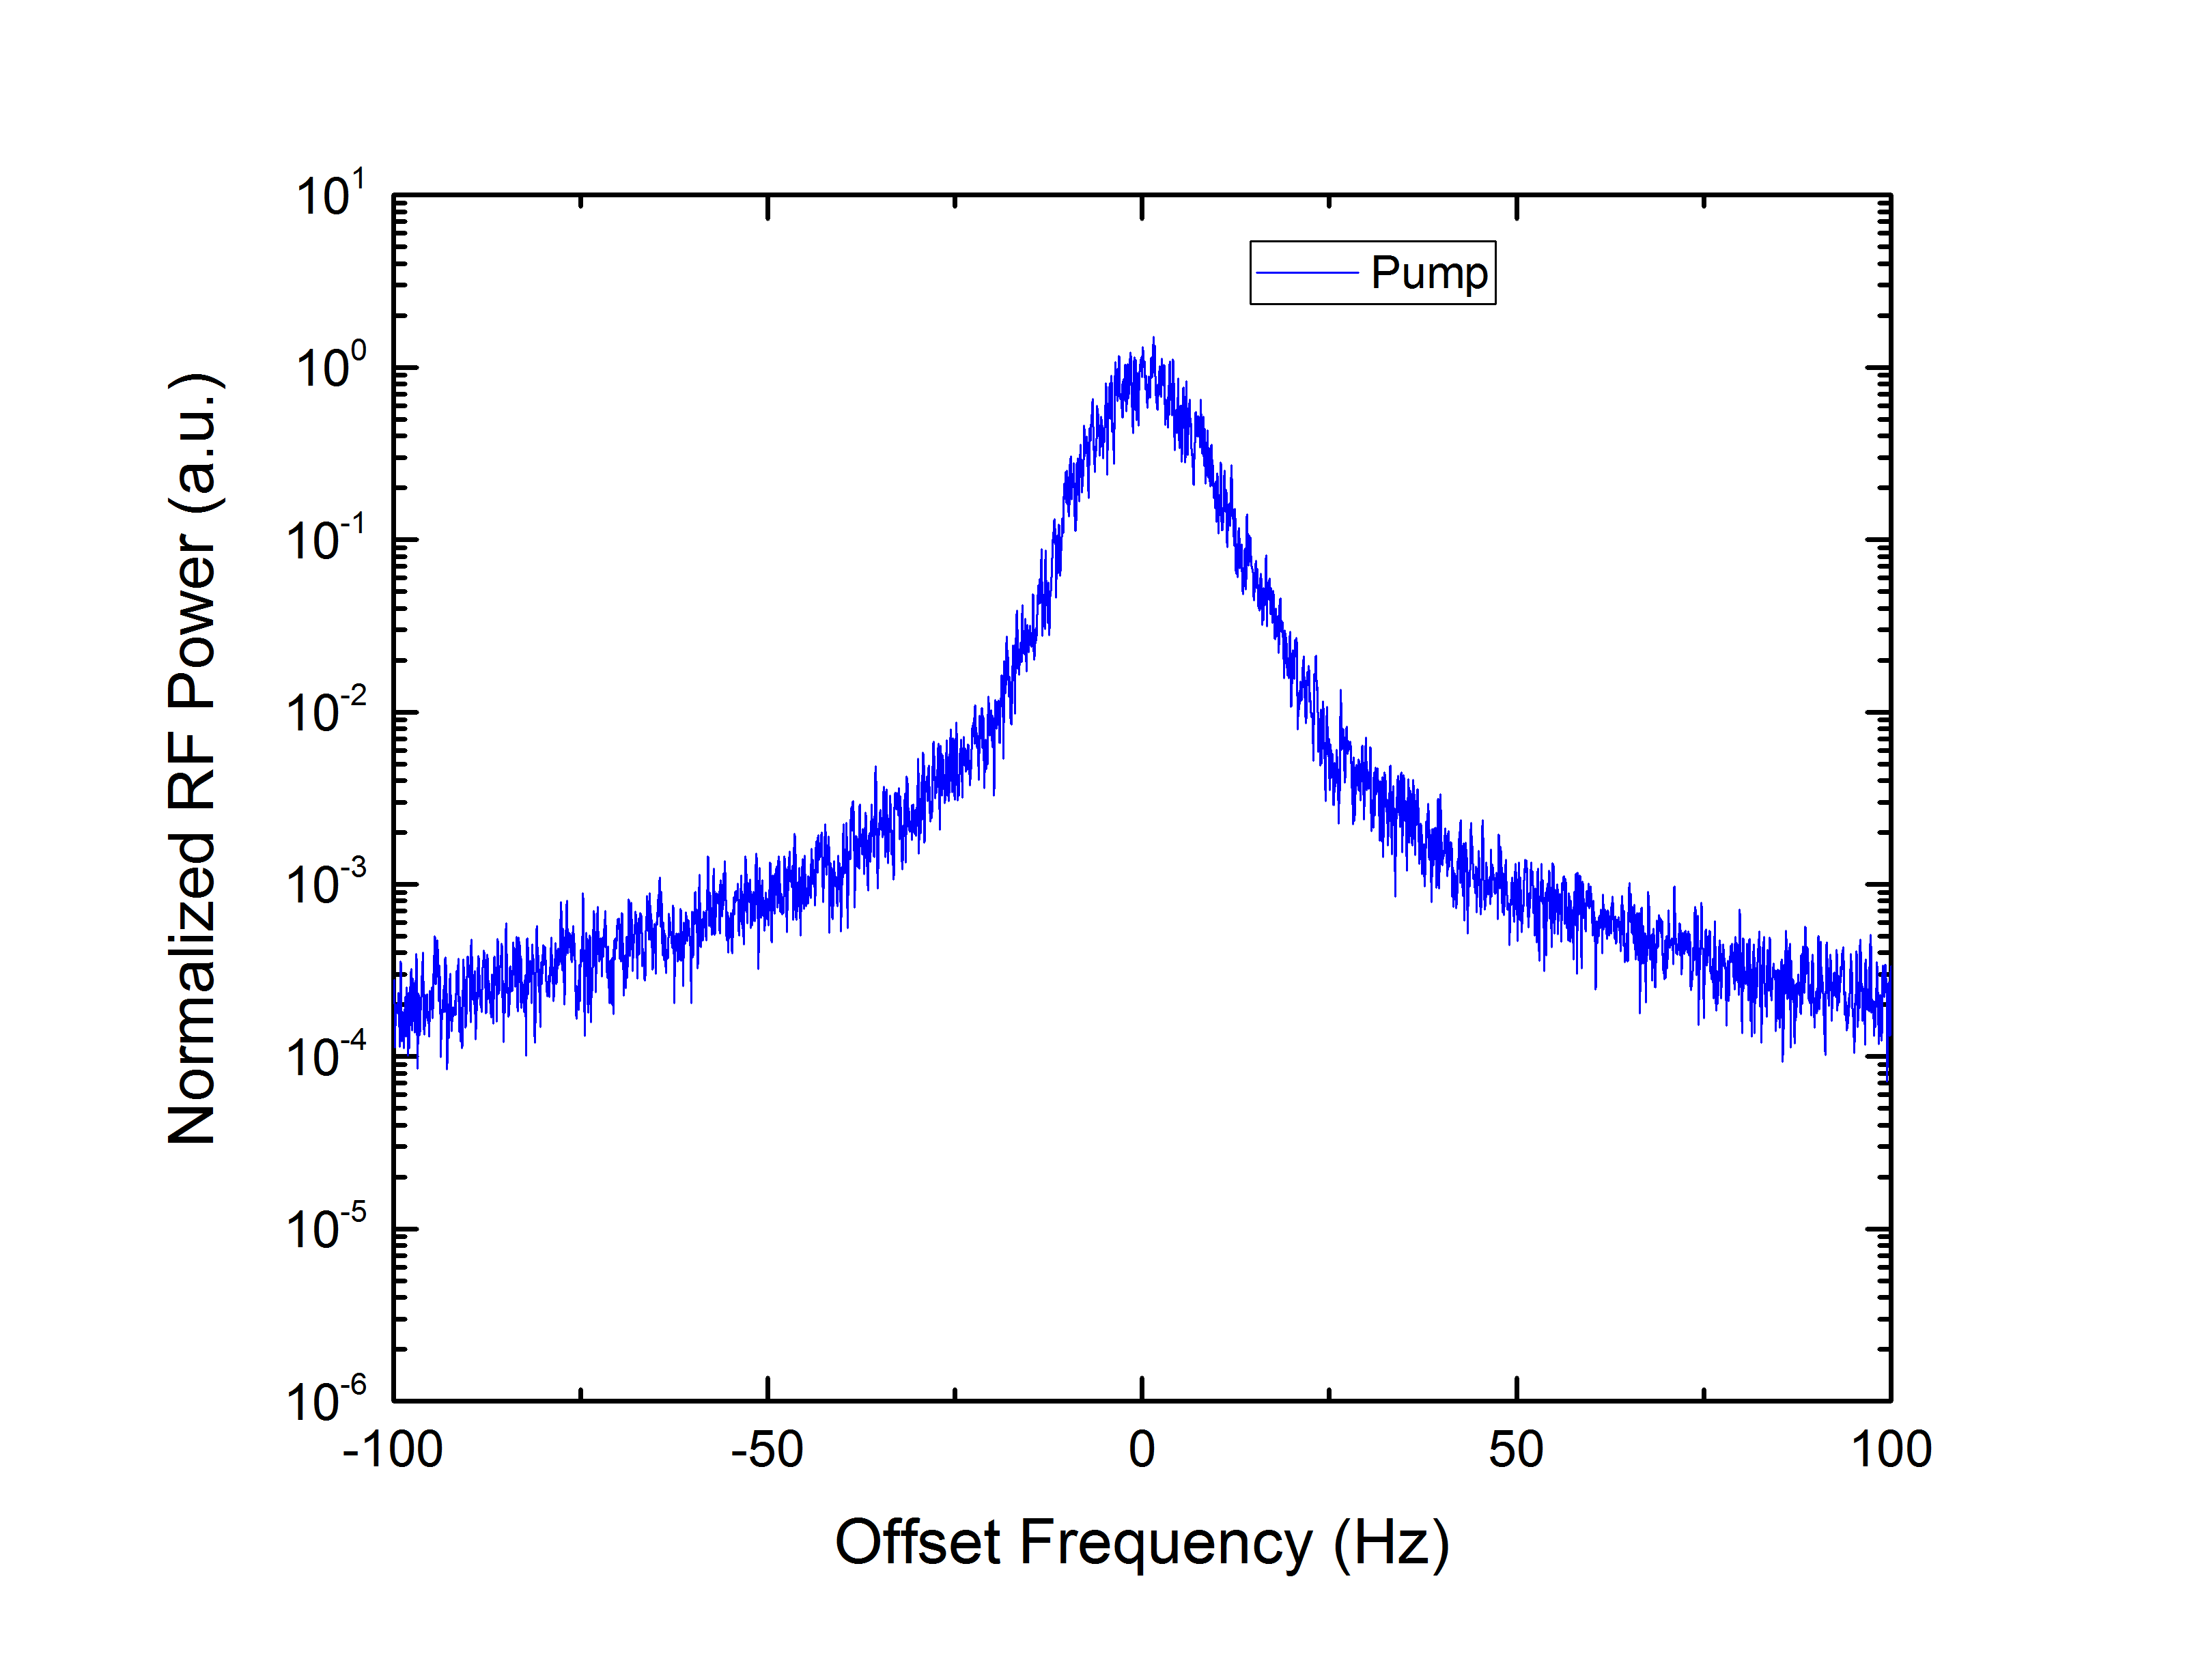
\includegraphics[width=1.0\textwidth]{Images/RF_Spectrum_Plot1.png}

\column{0.5\textwidth}
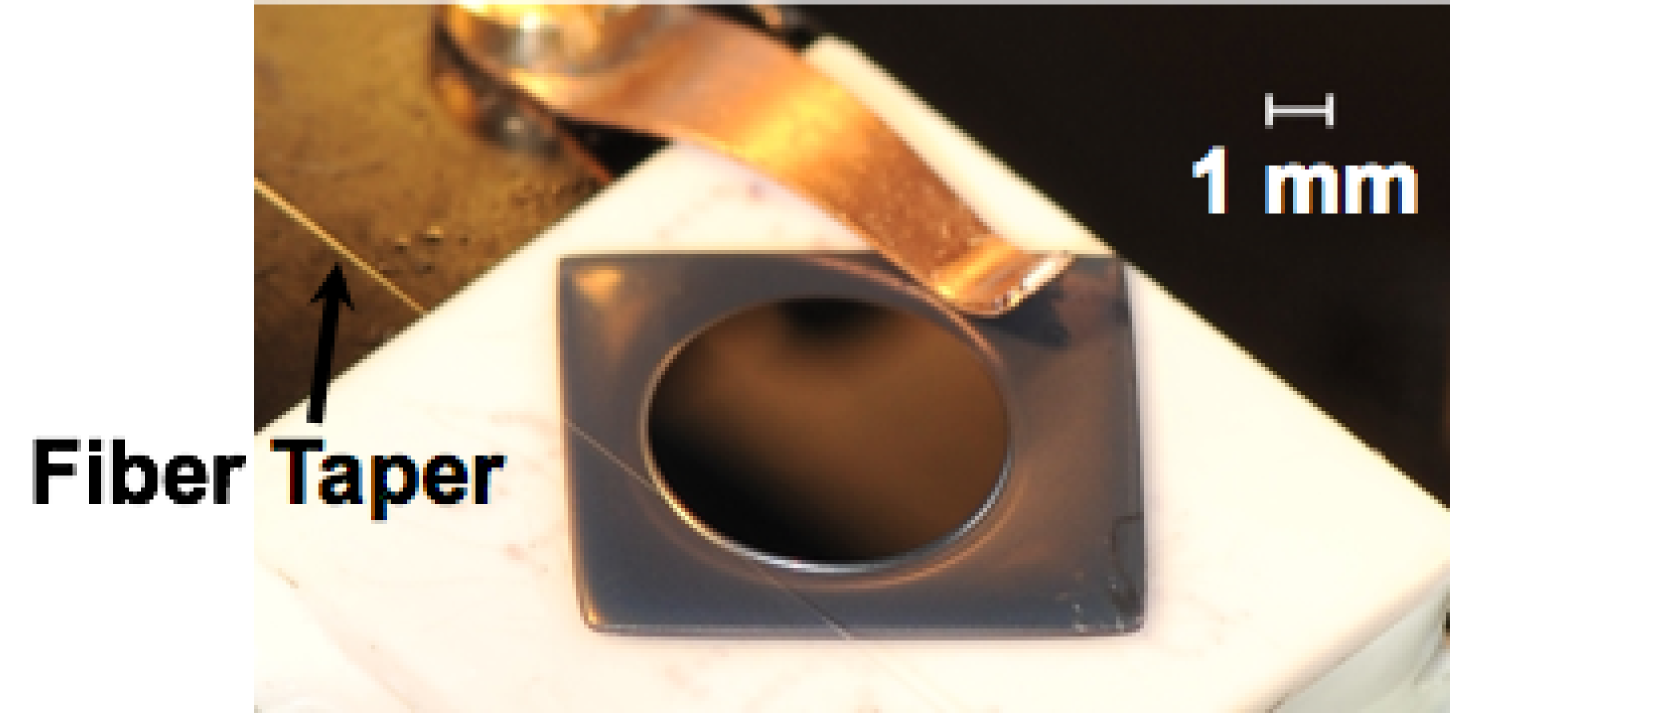
\includegraphics[width=0.9\textwidth]{Images/Microdisk.png}\\
\begin{block}{Previous Microdisk Work}
\begin{itemize}
\item We measured a reduction in noise level by generating an SBS laser within a microdisk.
\item This system has been shown to be tunable up to THz.
\item This SBS laser has be referenced to a cavity for further noise reduction.
\end{itemize}
\end{block}
\end{columns}
\end{frame}

\begin{frame}\frametitle{Increasing Mode Volume}

\begin{block}{Moving from a Microdisk to a Microrod}
\begin{columns}
\column{0.3\textwidth}
\begin{itemize}
\item Microdisk thickness of $\approx 10\mu m$ 
\linebreak
\linebreak
\linebreak
\linebreak
\linebreak
\item Microrod thickness of $\approx 100\mu m$
\end{itemize}

\column{0.3\textwidth}
\begin{center}
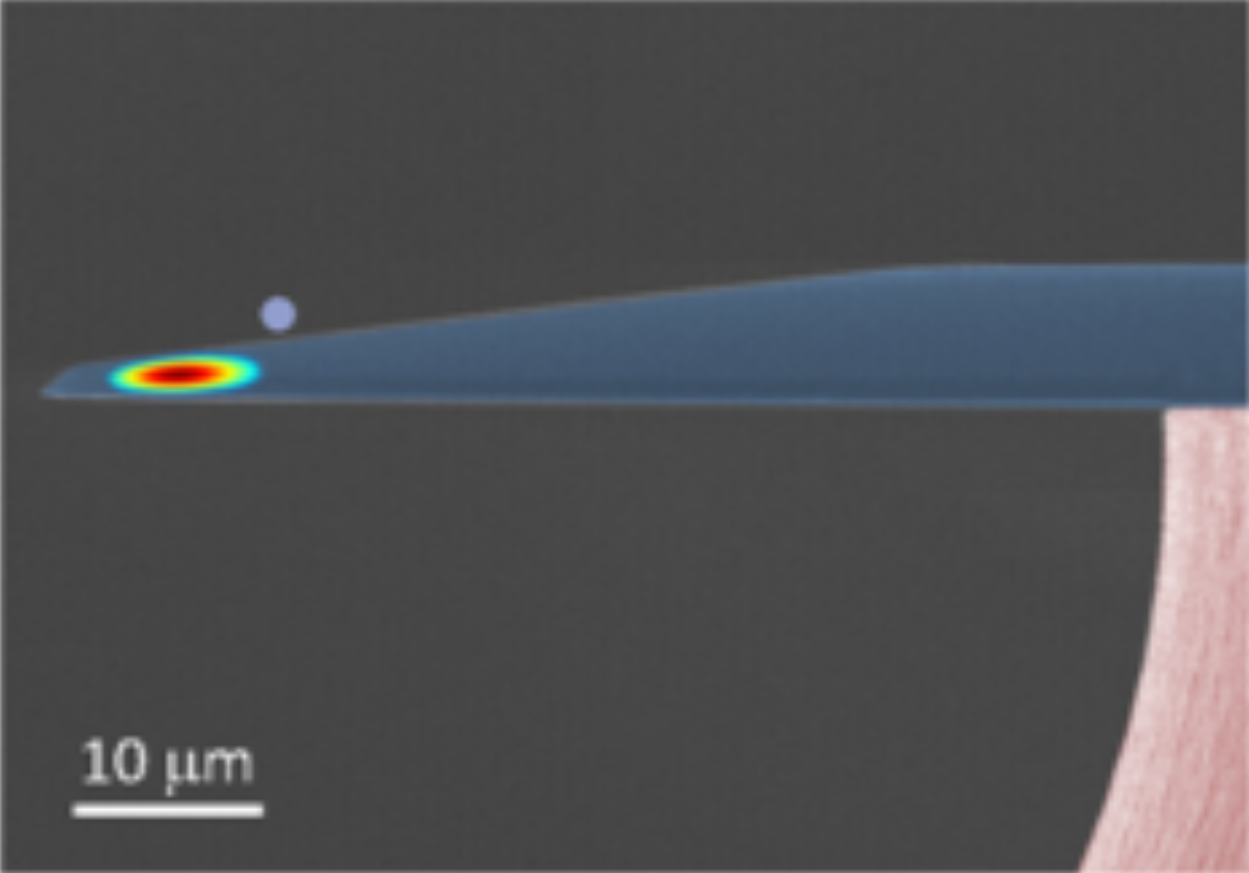
\includegraphics[width=0.9\textwidth]{Images/Microdisk_Profile.png}\\
\footnotesize{H. Lee, Nature Photonics, 2012}\\
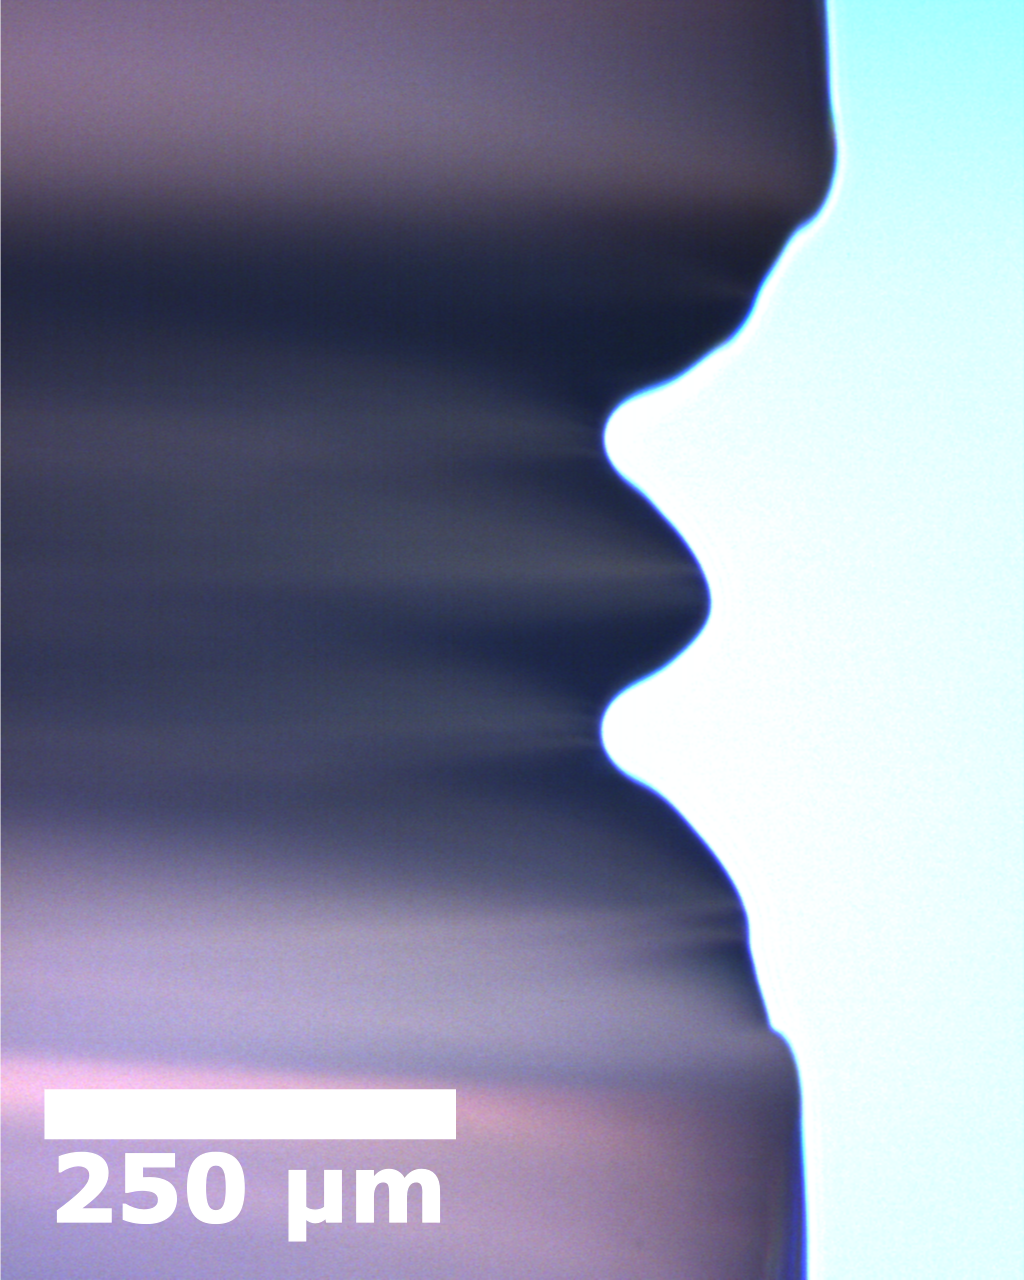
\includegraphics[width=1.0\textwidth,keepaspectratio]{Images/Microrod_Profile.png}
\end{center}

\column{0.3\textwidth}
$$S_{\bar{u}}(\Omega)\propto V_m^{-1}$$\\

\footnotesize{A. Matsko, J. Opt. Soc. Am. B, 2007}\\

\begin{itemize}
\item By increasing mode volume we reduce the amount of thermal fluctuations.
\end{itemize}

\end{columns}
\end{block}
\end{frame}

\begin{frame}\frametitle{Silica Microrod Resonators}
\includemedia[
  width=1.0\textwidth,
  height=1.0\textheight,
  activate=onclick,
  addresource=Microrod_Fabrication.mp4,
  flashvars={flv=Microrod_Fabrication.mp4&autoPlay=true}]{
  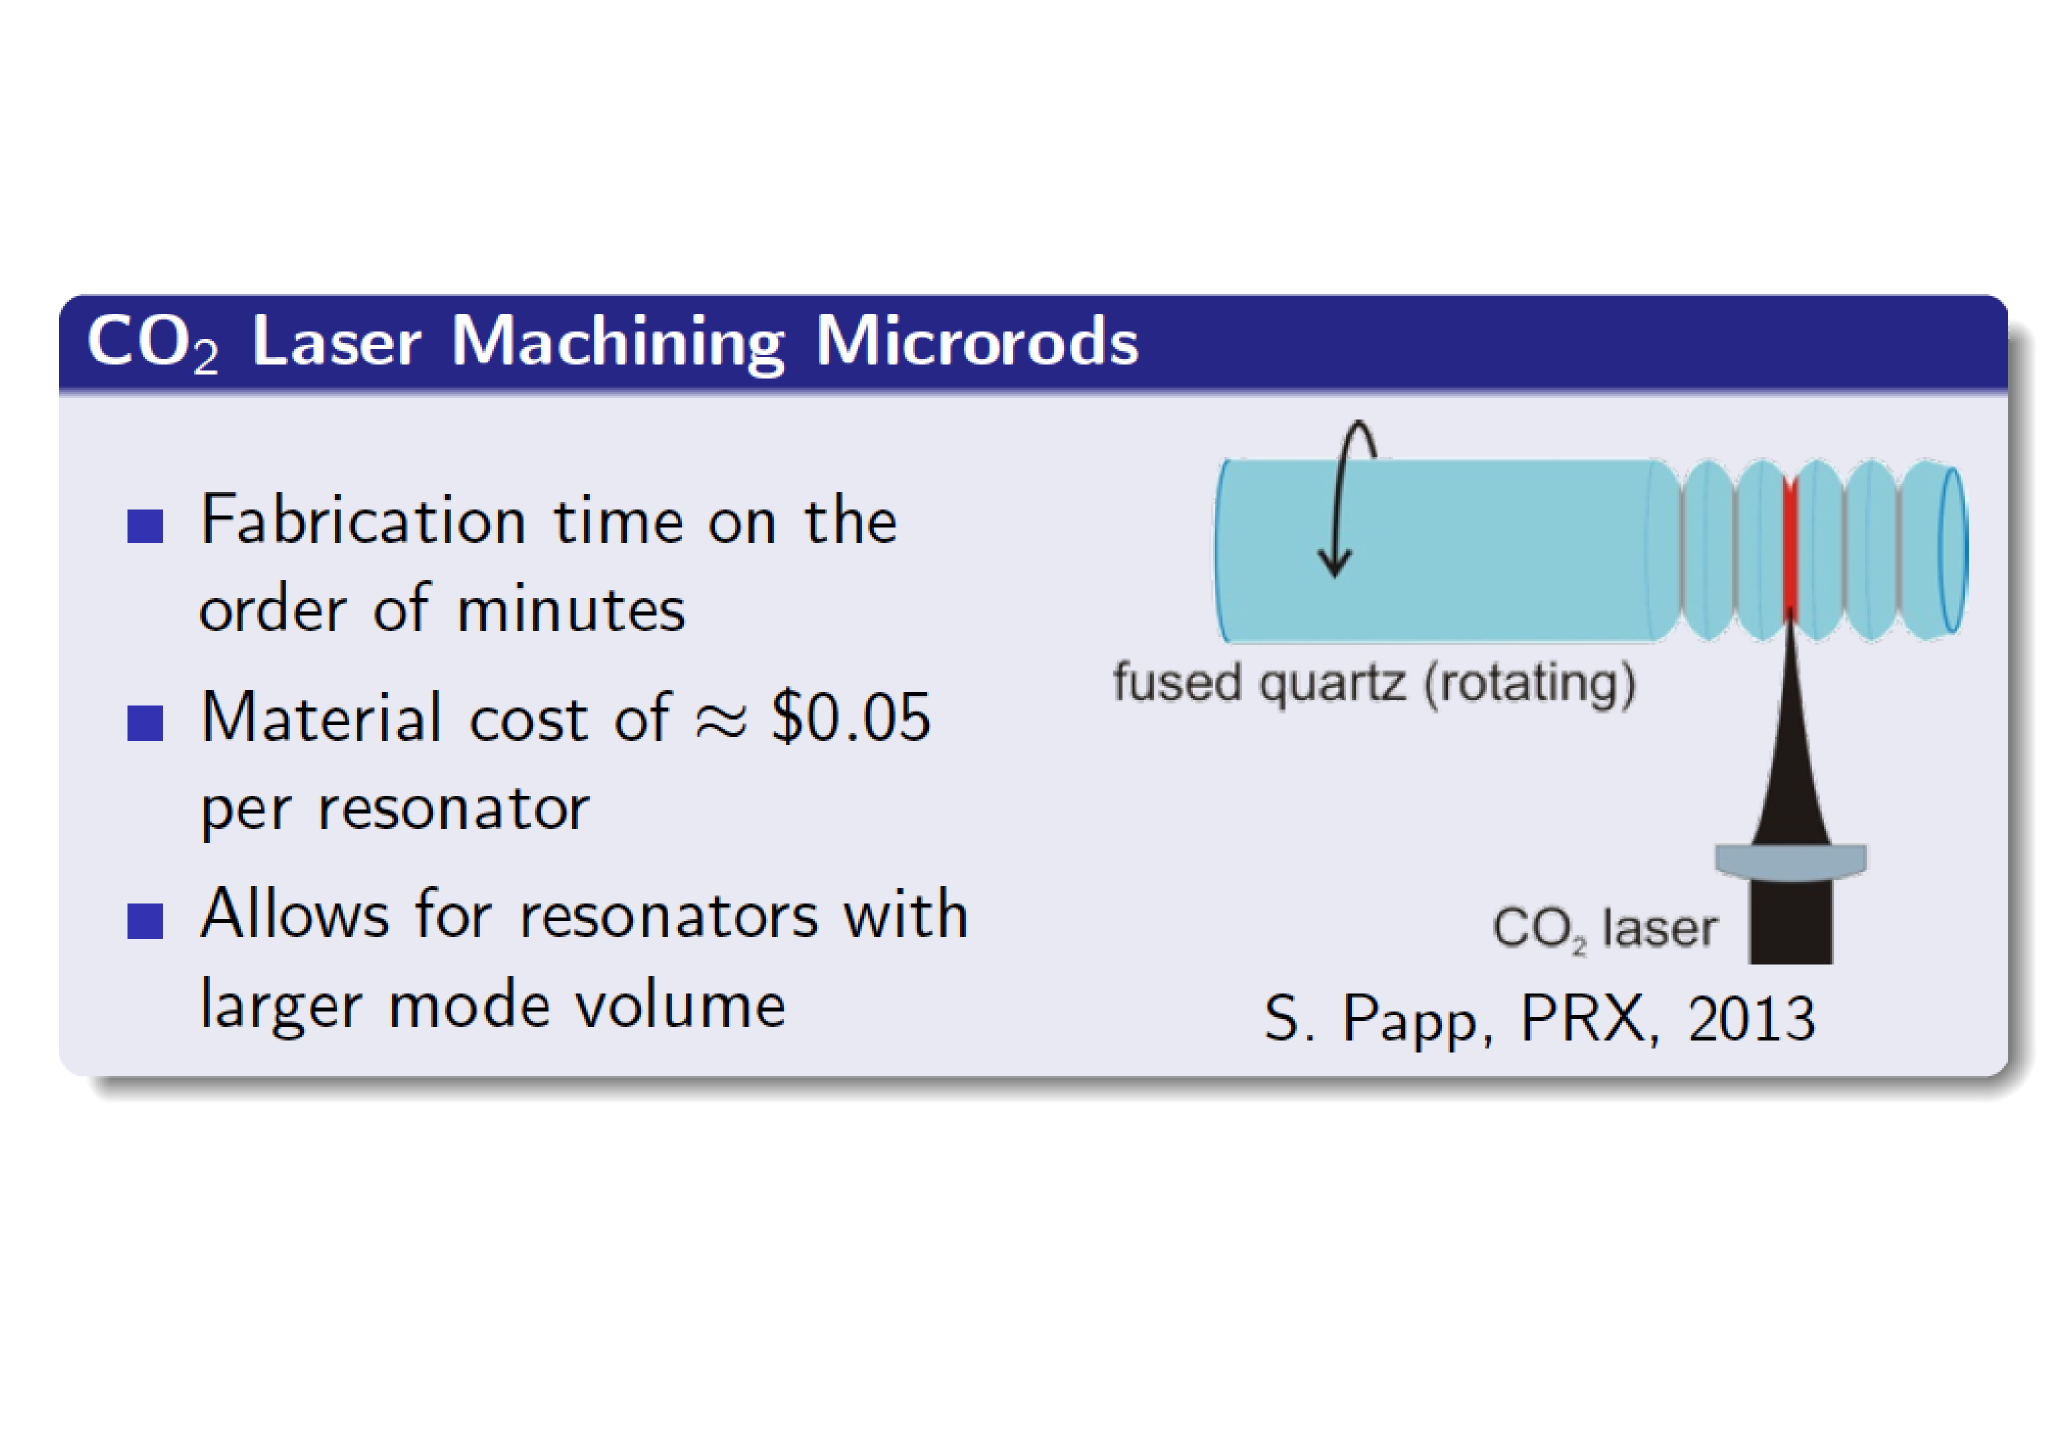
\includegraphics[width=1.0\textwidth]{Images/Laser_Machine_Fig.png}
}{player_flv_maxi.swf}
\end{frame}

\section{Experiment}

\begin{frame}\frametitle{Apparatus}
\begin{columns}
\column{0.5\textwidth}
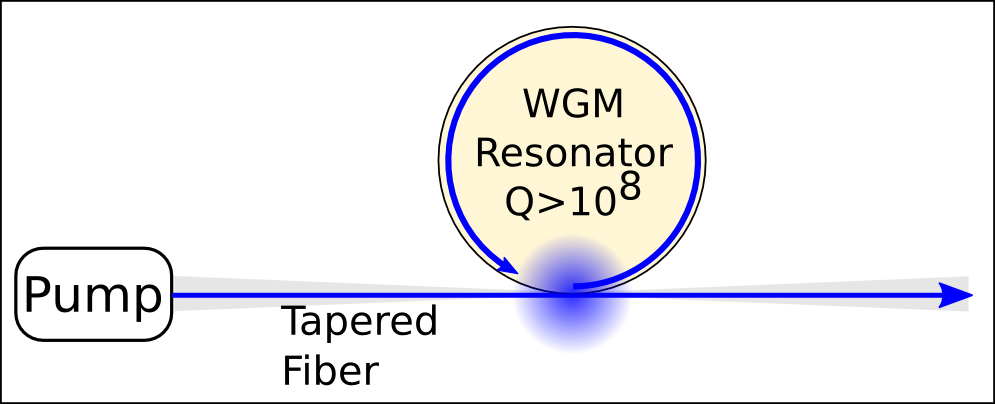
\includegraphics[width=1.0\textwidth]{Images/WGM_Resonator_Fig.png}\\
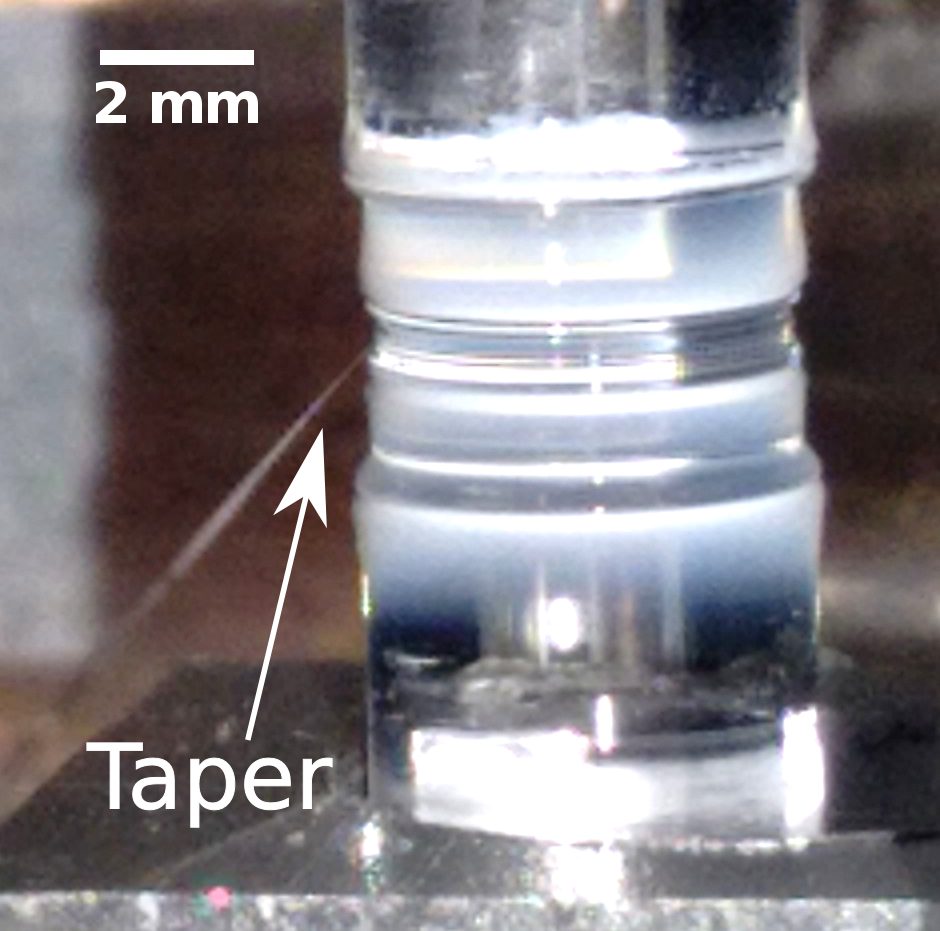
\includegraphics[width=1.0\textwidth]{Images/SBS_Microrod.png}
\column{0.5\textwidth}
\begin{block}{Fiber Coupling}
\begin{itemize}
\item We pull a single mode optical fiber to form a taper with a waist on the order of the wavelength our light.
\item With a fiber smaller than the optical mode we are able to overlap modes between the taper and the resonator. 
\item This allows for a simple fiber integrated system.
\end{itemize}
\end{block}
\end{columns}
\end{frame}

\section{Results}
\begin{frame}\frametitle{SBS Microrod Laser Frequency Noise}
\includegraphics<1>[width=1.0\textwidth]{Images/Freq_Noise_Comparison_Plot1.png}
\includegraphics<2>[width=1.0\textwidth]{Images/Freq_Noise_Comparison_Plot2.png}
\end{frame}

\begin{frame}\frametitle{SBS Microrod Laser RF Spectrum}
\includegraphics<1>[width=1.0\textwidth]{Images/RF_Spectrum_Plot1.png}
\includegraphics<2>[width=1.0\textwidth]{Images/RF_Spectrum_Plot2.png}
\end{frame}

\section{Conclusions}
\begin{frame}\frametitle{Summary of Results}
\begin{itemize}
\item We observed a two order reduction in noise from the SBS microdisk by changing to the microrod
\item We observed an order reduction in linewidth from the SBS microdisk as well
\end{itemize}

\begin{block}{Future Research Directions}
\begin{columns}
\column{0.4\textwidth}
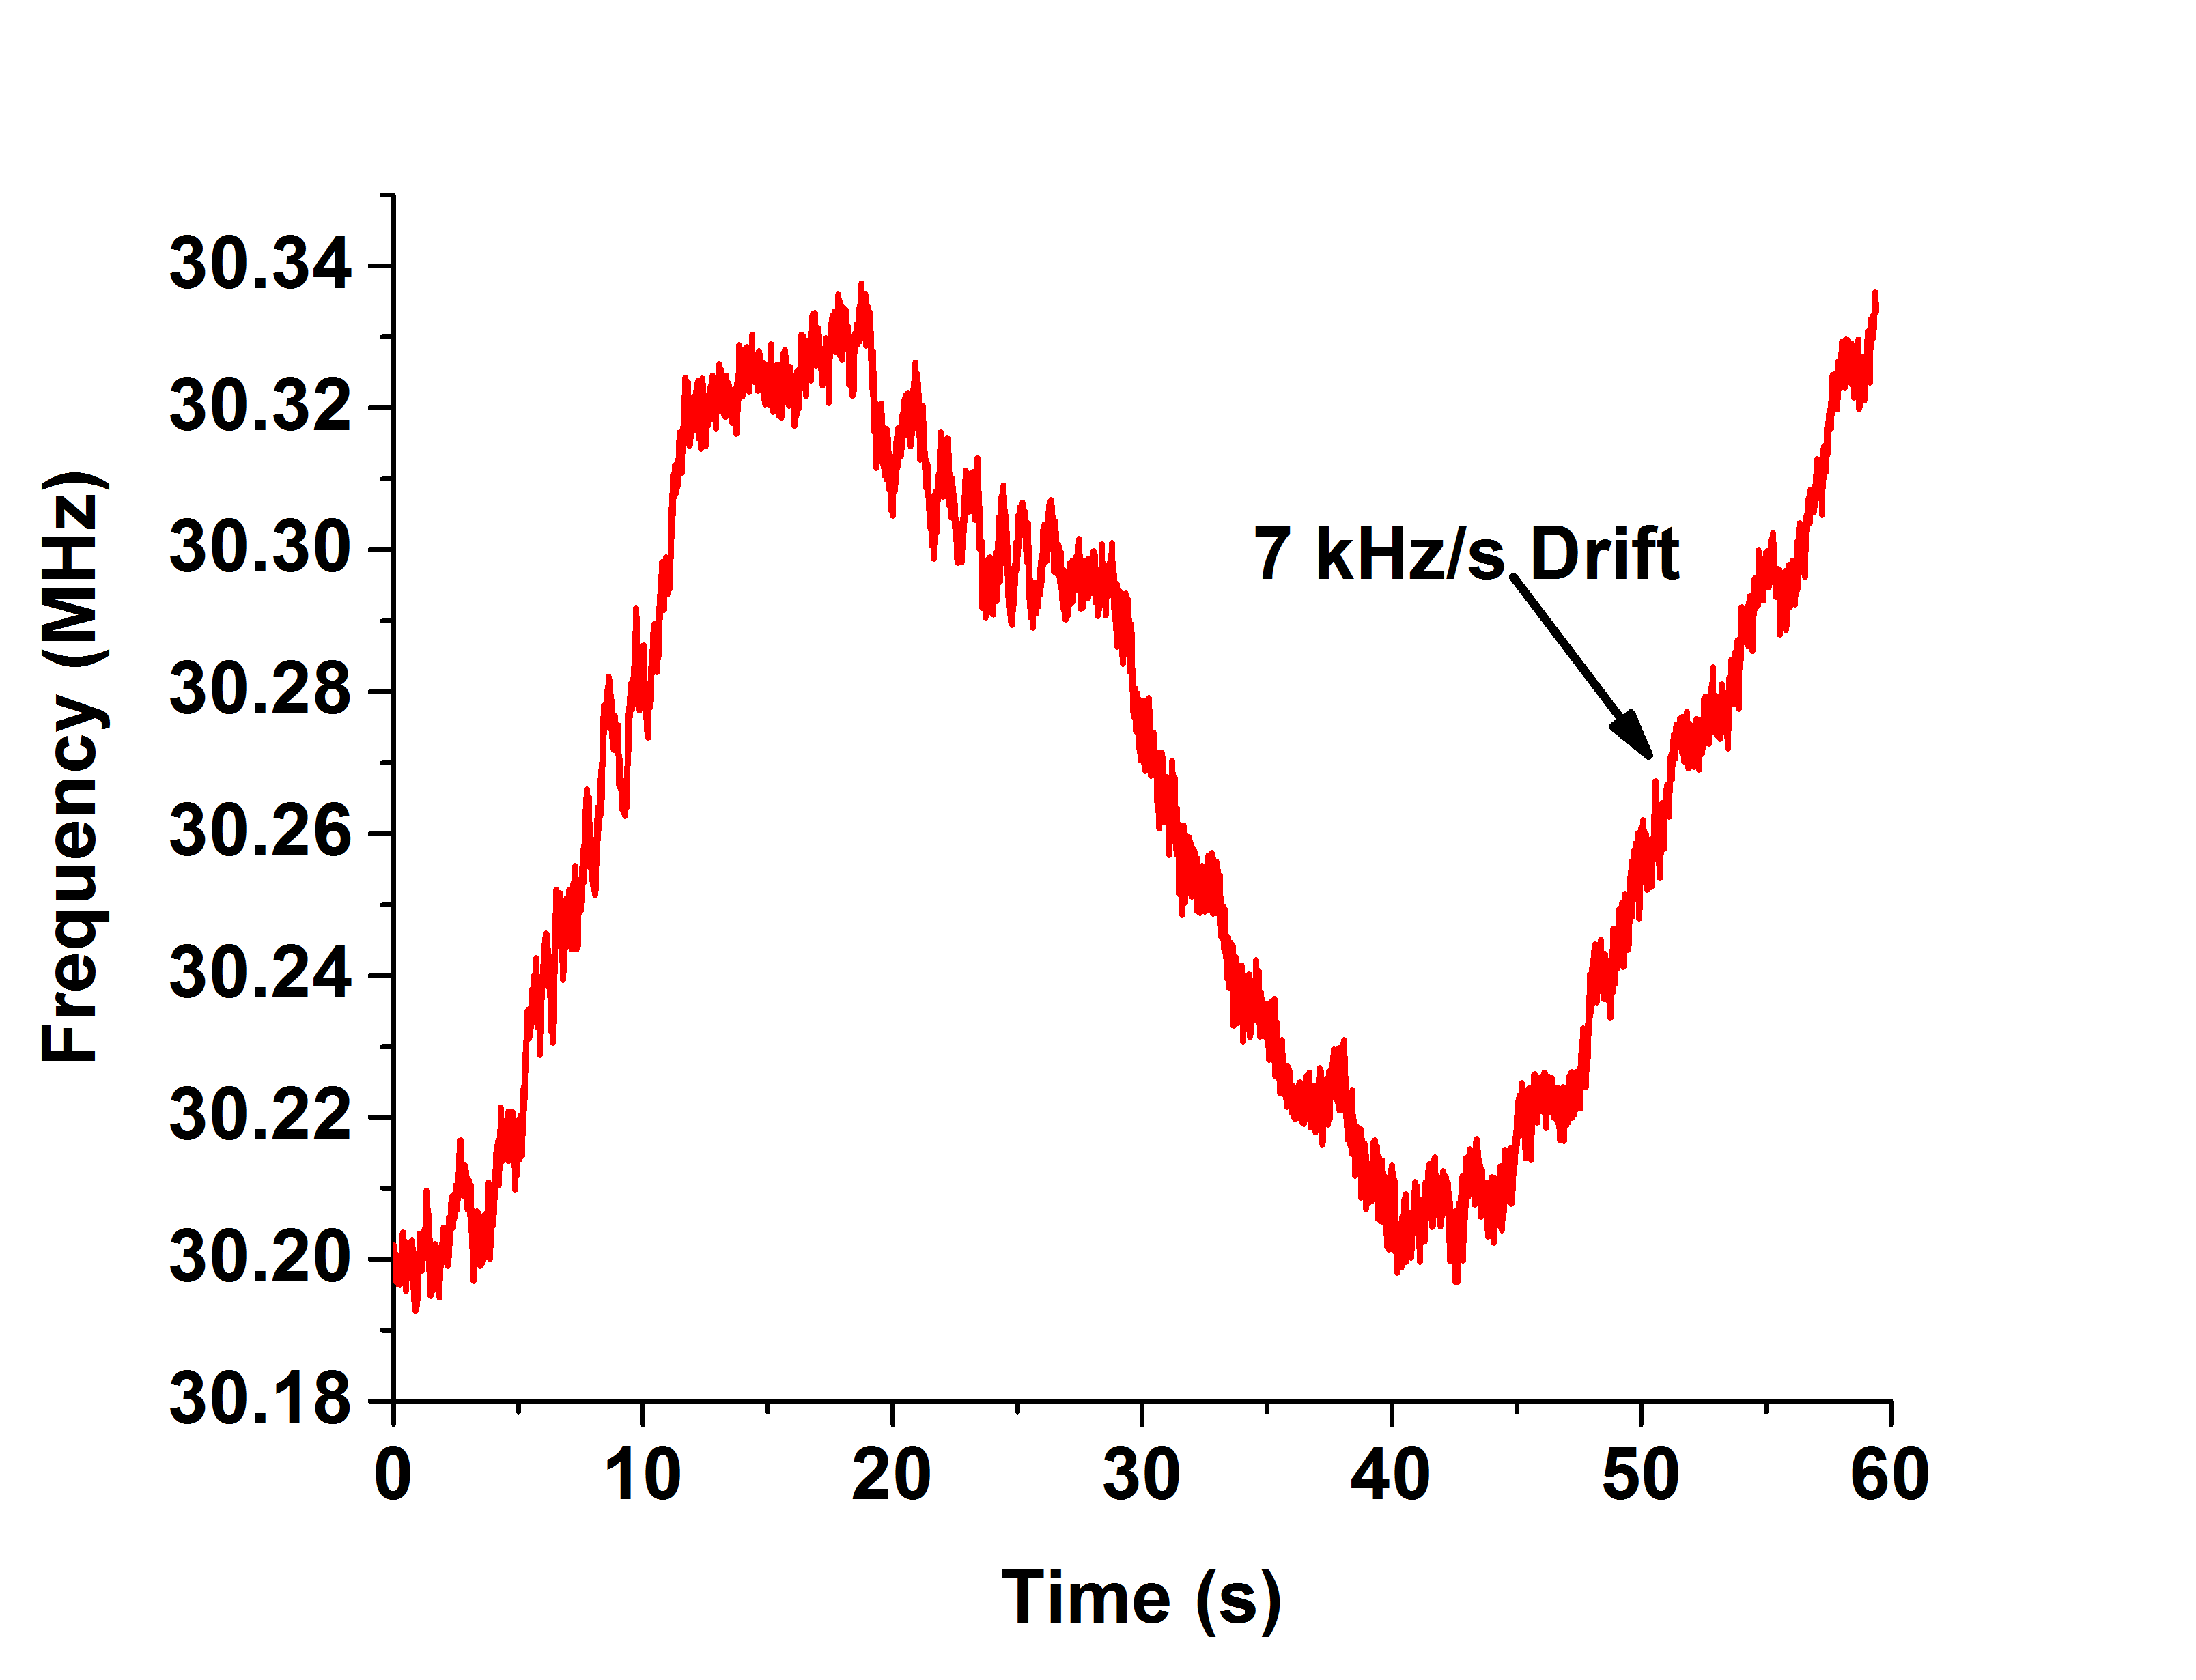
\includegraphics[width=0.95\textwidth]{Images/Thermal_Drift.png}
\column{0.5\textwidth}
\begin{itemize}
\item We have observed a free running thermal drift of $7kHz/s$ and would like to make efforts to reduce the drift.
\end{itemize}
\end{columns}

\end{block}
\end{frame}

\begin{frame}\frametitle{Acknowledgments}
A special thanks to:
\begin{columns}
\column{0.5\textwidth}
\begin{block}{\centering The NIST Optical Frequency Measurement Lab}
\begin{itemize}
\small
\item Fred Baynes
\item Katja Beha
\item Aur\'{e}lien Coillet
\item Daniel Cole
\item Pascal Del'Haye
\item Scott Diddams
\item Adam Green
\item William Loh
\item Scott Papp
\item Frank Quinlan
\end{itemize}
\end{block}

\column{0.5\textwidth}
\begin{block}{\centering The Caltech Vahala Group}
\begin{itemize}
\small
\item Hansuek Lee
\item Kerry Vahala
\end{itemize}
\end{block}

\begin{block}{\centering Funding Provided By}
\begin{center}
\small
The DARPA PULSE Program

\includegraphics[width=1.1\textwidth]{Images/DARPA_logo.png}
\end{center}
\end{block}

\end{columns}
\end{frame}

\begin{frame}\frametitle{Questions?}
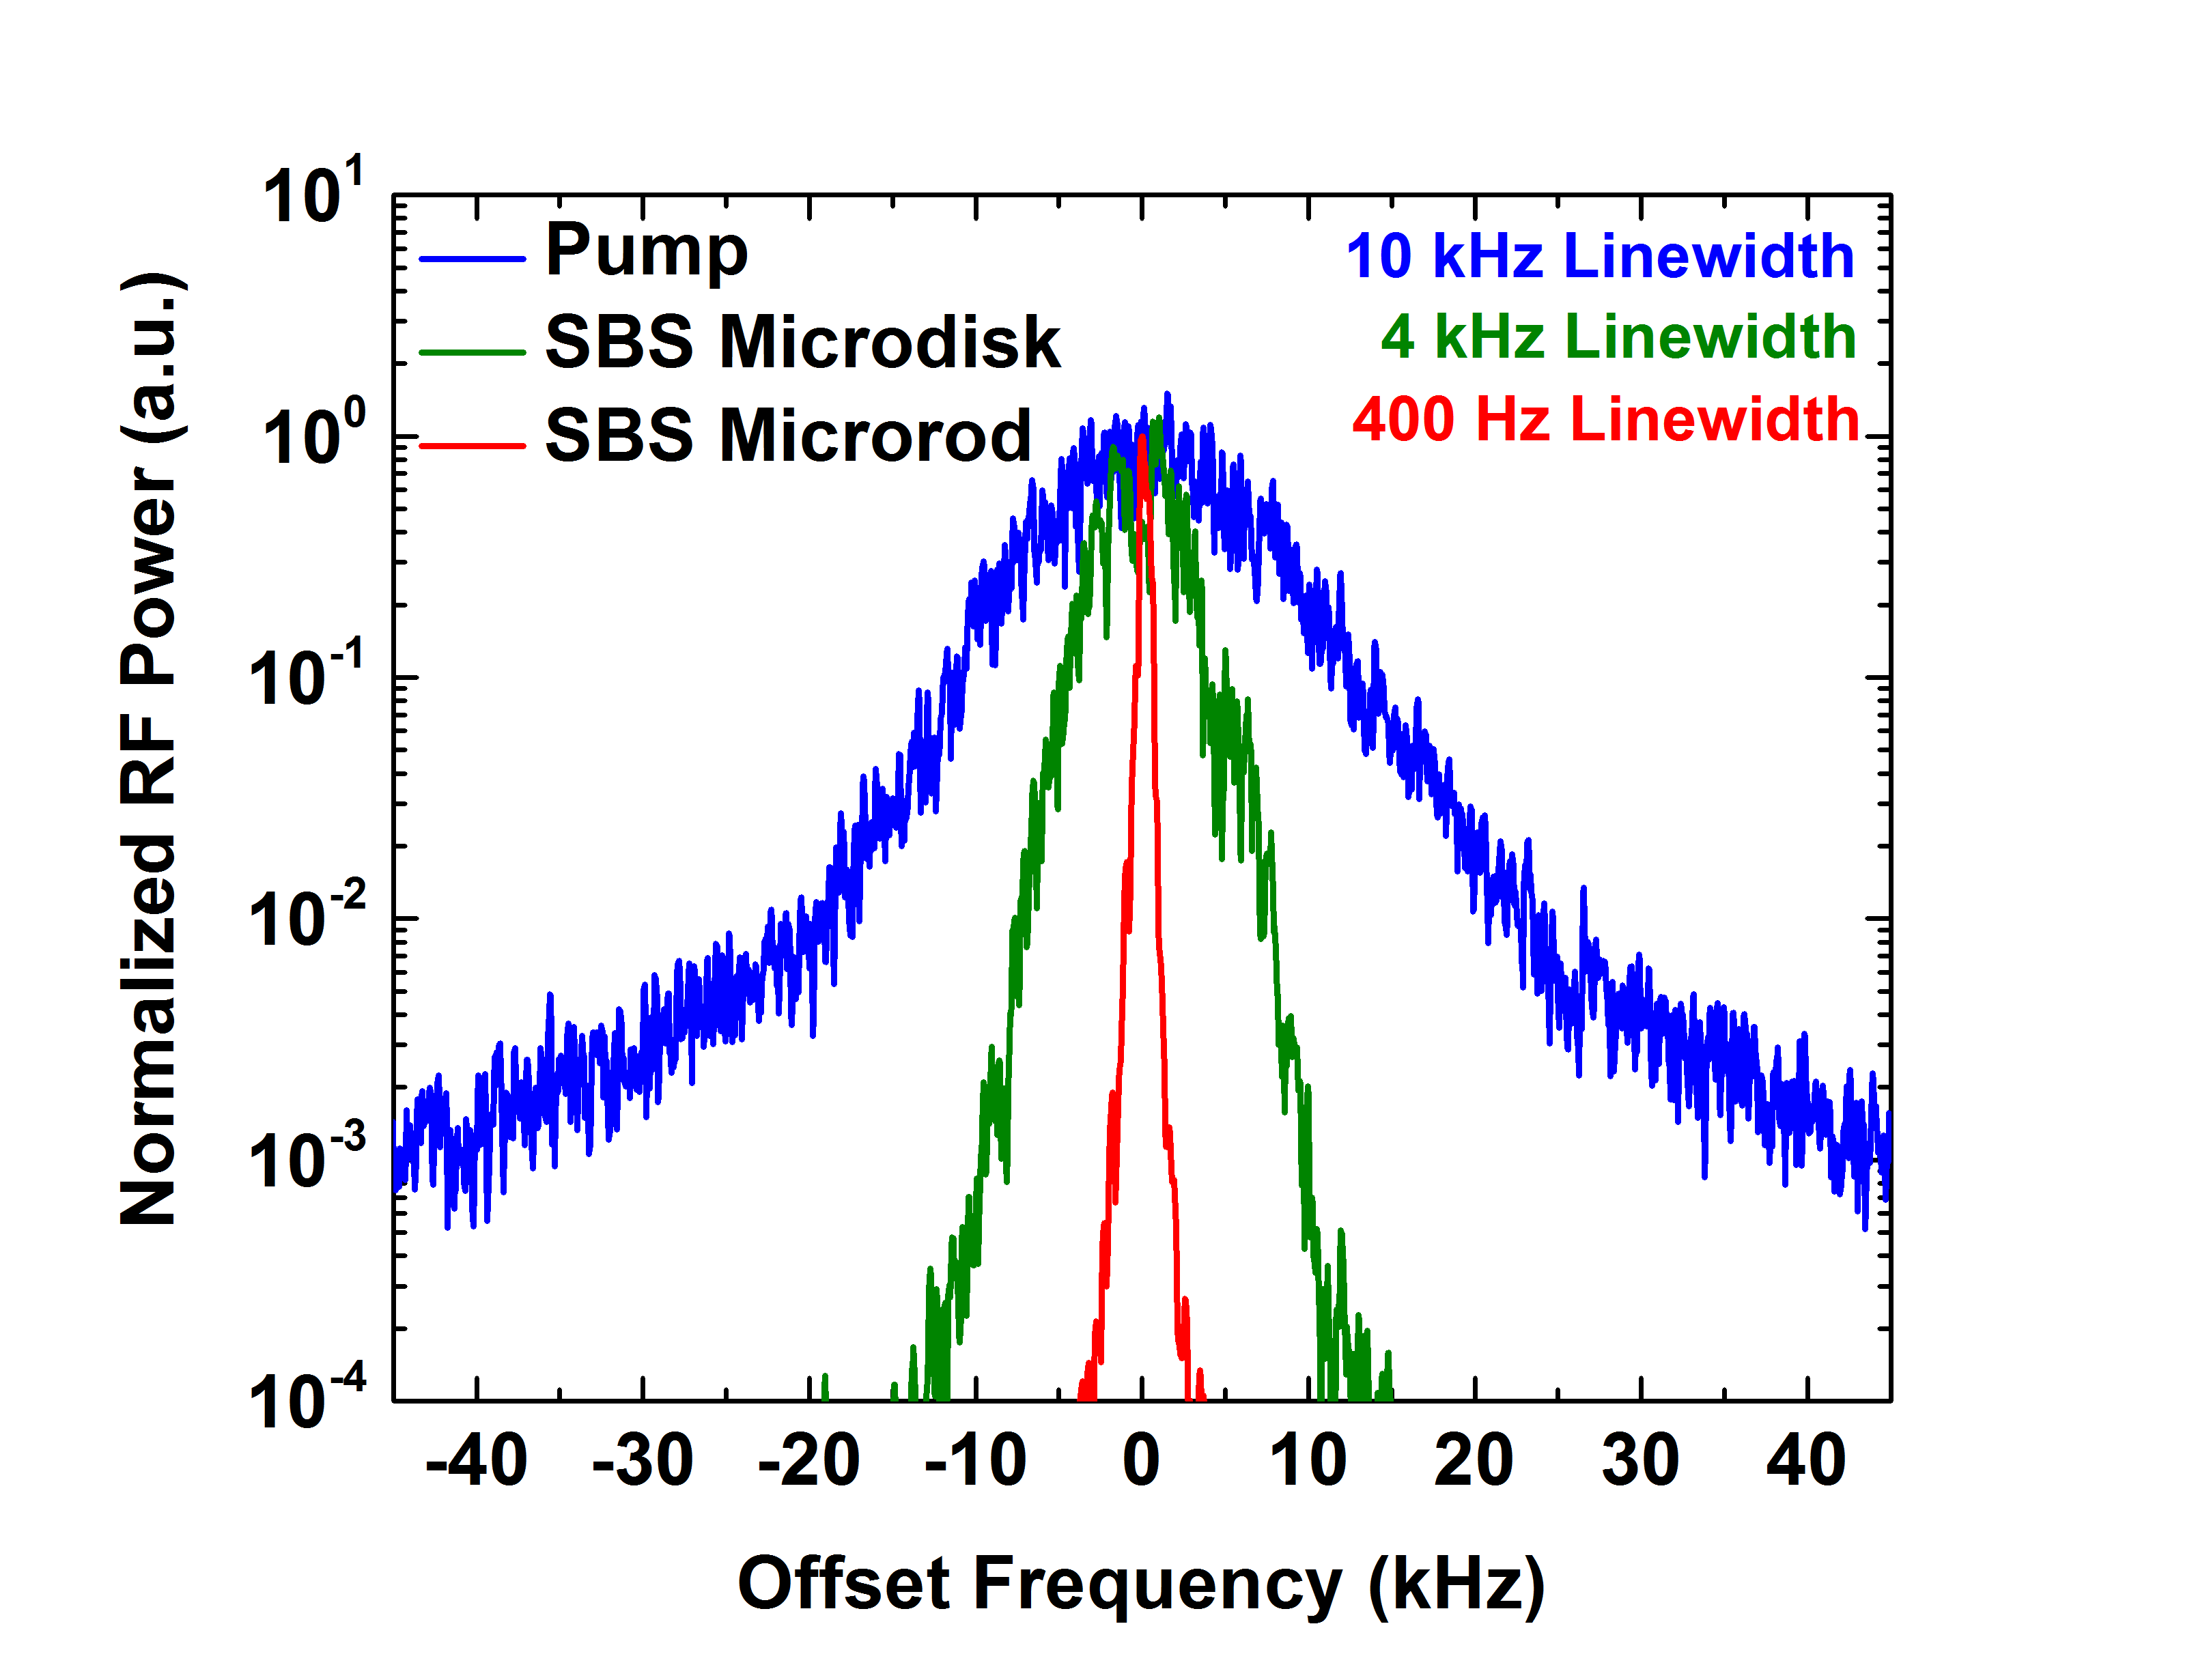
\includegraphics[width=1.0\textwidth]{Images/RF_Spectrum_Plot2.png}
\end{frame}

\end{document} 
